\documentclass[a4paper]{book}
%11pt,a4paper,twoside
\usepackage{polski}
\usepackage[utf8]{inputenc}
\usepackage[titletoc]{appendix}
\usepackage{tikz}
\usepackage{indentfirst}
\usepackage{comment}
\PassOptionsToPackage{hyphens}{url}
\usepackage{hyperref}
\usepackage{breakurl}
\usepackage{mathtools}
\usepackage{wasysym} % symbole astronomiczne
 
\frenchspacing

%%%% TODO LIST GENERATOR %%%%%%%%%

%\usepackage{tikz}
\usepackage{manfnt}   % dangerous sign 
\usepackage{color}
\definecolor{brickred}      {cmyk}{0   , 0.89, 0.94, 0.28}

\makeatletter \newcommand \kslistofremarks{\section*{Uwagi} \@starttoc{rks}}
  \newcommand\l@uwagas[2]
    {\par\noindent \textbf{#2:} %\parbox{10cm}
{#1}\par} \makeatother


\newcommand{\ksremark}[1]{%
{\marginpar{\textdbend}{\color{brickred}{[#1]}}}%
\addcontentsline{rks}{uwagas}{\protect{#1}}%
}

%%%%%%%%%%%%%% END OF TODO LIST GENERATOR %%%%%%%%%%%


% ustawienia marginesow
%\usepackage[cm]{fullpage}
%\usepackage[top=2.5cm, bottom=2.5cm, inner=3.5cm, outer=2.5cm, twoside]{geometry}

% ustawienia obrazow %
\usepackage{graphicx}
\usepackage{caption}
\usepackage{subcaption}

\graphicspath{ {./assets/} }
\DeclareGraphicsExtensions{.pdf,.png,.jpg}

%nazwa aplikacji
\newcommand{\appName}{\emph{TravelGuide}}
%czy mogę zmienić nazwę aplikacji na "TravelGuide" zamiast "Wirtualny Przewodnik"? Czyli tak, jak jest logo, etc.?


% listing kodu
\usepackage{listings}
\usepackage{color}

\lstloadlanguages{
	csh
}

\definecolor{red}{rgb}{0.6,0,0} % for strings
\definecolor{blue}{rgb}{0,0,0.6}
\definecolor{green}{rgb}{0,0.8,0}
\definecolor{cyan}{rgb}{0.0,0.6,0.6}

\lstset{
	language=csh,
	basicstyle=\footnotesize\ttfamily, 
	numbers=left, 
	numberstyle=\tiny, 
	numbersep=5pt, 
	tabsize=2, 
	extendedchars=true, 
	breaklines=true, 
	frame=b,
	stringstyle=\color{blue}\ttfamily, 
	showspaces=false, 
	showtabs=false, 
	xleftmargin=17pt,
	framexleftmargin=17pt,
	framexrightmargin=5pt,
	framexbottommargin=4pt,
	commentstyle=\color{green},
	morecomment=[l]{//}, %use comment-line-style!
	morecomment=[s]{/*}{*/}, %for multiline comments
	showstringspaces=false, 
	morekeywords={  abstract, event, new, struct,
		as, explicit, null, switch,
		base, extern, object, this,
		bool, false, operator, throw,
		break, finally, out, true,
		byte, fixed, override, try,
		case, float, params, typeof,
		catch, for, private, uint,
		char, foreach, protected, ulong,
		checked, goto, public, unchecked,
		class, if, readonly, unsafe,
		const, implicit, ref, ushort,
		continue, in, return, using,
		decimal, int, sbyte, virtual,
		default, interface, sealed, volatile,
		delegate, internal, short, void,
		do, is, sizeof, while,
		double, lock, stackalloc,
		else, long, static,
		enum, namespace, string, var},
	keywordstyle=\color{cyan},
	identifierstyle=\color{red},
}

% document settings
\begin{document}	

\kslistofremarks

\cleardoublepage
%stara strona tytułowa
\begin{comment}
	\begin{titlepage}
		\begin{center}
			
\includegraphics[width=4cm]{assets/images/polsl.jpg}\\[1cm]
			\textsc{\LARGE{Politechnika Śląska}}\\[0.5cm]
			\textsc{\LARGE{Wydział Automatyki, Elektroniki i~Informatyki}}\\[0.5cm]
			\textsc{\LARGE{Kierunek Informatyka}}\\[2.5cm]
			\LARGE{Projekt inżynierski}\\[1cm]
			\begingroup
			\fontsize{14pt}{17pt}\selectfont
		Wirtualny przewodnik dla urządzeń mobilnych
			\endgroup
		\end{center}
		\vspace{5cm}
		\begingroup
		\fontsize{14pt}{17pt}\selectfont
		\textbf{Autor:} Katarzyna Biernat\\
		\textbf{Kierujący pracą:} dr inż. Krzysztof Simiński\\
		\endgroup
		
		\vspace{3.5cm}
		\begingroup
		\fontsize{12pt}{14pt}\selectfont
		\begin{center}
			Gliwice, styczeń 2015
		\end{center}
		\endgroup
	\end{titlepage}
\end{comment}

%%%%%%%%   front.tex


% *************** Strona tytu³owa ***************
\pagestyle{empty}
\sffamily

\noindent
\begin{center}
    \Large
    Politechnika Śląska\\
    Wydział Automatyki, Elektroniki i Informatyki
    %\\ Nazwa kierunku
\end{center}

\begin{figure}[h]
\begin{center}

\includegraphics[width=0.2\textwidth]{images/polsl.pdf}
\end{center}
\end{figure}

\vfill\vfill
\begin{center}
    \Large
    Katarzyna Biernat
\end{center}

\vfill
\begin{center}
    \Huge\bfseries
    Wirtualny przewodnik dla urządzeń mobilnych
\end{center}

\vfill
\begin{center}
    \Large
    projekt inżynierski
\end{center}

\vfill\vfill\vfill
\begin{center}
    \Large
    Promotor/kierujący pracą: dr inż. Krzysztof Simiński
\end{center}

\vfill
\begin{center}
\large
   Gliwice, \today
\end{center}

\cleardoublepage

%% *************** Dedykacja ***************
%\vspace*{\fill}
%{\hfill\sffamily\itshape Pracę dedykuję \ldots}
%\cleardoublepage

\rmfamily
\normalfont

% *************** Spis treœci ***************
\pagenumbering{Roman}
\pagestyle{headings}
\tableofcontents

% *************** Koniec front matter ***************


%%%%%%%%  end of front

	
\mainmatter % powoduje, ze wlasciwa czesc pracy ma strony numerowe od 1 cyframi arabskimi
	
	\chapter{Wstęp}
	\label{id:cha:wstep}
		 
			Ludzi od lat fascynowały dalekie podróże i nieznane lądy. Już starożytni zastanawiali się co znajduje się za wielką wodą. Chyba każdy ze szkoły zna opowieść o mitycznym Odyseuszu i jego wyprawie autorstwa Homera czy też \textit{Anabazę} pióra Ksenofonta opisującą brawurowy powrót greckiego wojska najemnego spod Kunaksy w Babilonii do Grecji. Kiedy w czasach renesansu pojawiła się ku temu możliwość, ludzie wsiedli na statki i wypłynęli w szerokie morze w poszukiwaniu nowych, nieznanych terenów. I tak też w 1492 roku Krzysztof Kolumb dopłynął aż do Ameryki, a w 1519 Ferdynand Magellan wyruszył opłynąć cały świat. 
			
			Warto jednak wspomnieć, że jeszcze do niedawna podróże zarezerwowane były dla nielicznych. Ograniczeniem były  finanse i brak szybkich środków lokomocji, ale i ludzki strach przed nieznanym. Dopiero po 1945 roku \cite{id:historia_podrozy}, wraz z rozwojem motoryzacji, kolei i lotnictwa oraz ogólnym polepszeniem standardu życia, zagraniczne wakacje stały się popularne na skalę masową. Spowodowało to gwałtowną ekspansję branży turystycznej, na którą składają się nie tylko biura podróży czy hotele, ale i wydawnictwa podróżnicze wydające przewodniki turystyczne. 
			
			Branżą, która rozwija się jeszcze szybciej niż turystyka, jest branża IT. Jeszcze 10 lat temu nikomu nie śniło się, że dziś prawie każdy posiadać będzie telefon typu smartfon\footnote{ang. \emph{smartphone} -- dosłownie ,,mądry telefon''}. Turystyka nie nadąża za rozwojem IT, więc w chwili obecnej na rynku istnieje nisza, jeśli chodzi o przewodniki elektroniczne.
			
			Celem niniejszego projektu jest stworzenie przyjaznej platformy \appName\ dedykowanej dla osób podróżujących. Program ma ułatwić użytkownikowi zwiedzanie nowych miejsc oraz zupełnie zastąpić tradycyjny, książkowy przewodnik. Na całość składać się będzie aplikacja mobilna na platformę Windows Phone 8.1 oraz aplikacja działająca w przeglądarce internetowej. 
			
			W Internecie można znaleźć bardzo wiele różnych informacji o ciekawych miejscach turystycznych, brakuje jednak przyjaznej formy przedstawienia ich podróżnikowi. 
			
			Rysunek~\ref{fig:fly4freeAnkieta} przedstawia wyniki ankiety przeprowadzonej wśród 234 użytkowników forum Fly4Free.pl \cite{id:fly4free}. Jak się okazuje, zdecydowana większość podróżników zakupuje przewodnik o miejscu docelowym bądź pobiera stosowne informacje z sieci i drukuje je na swój użytek.
			
			Aplikacja \appName\ ma na celu połączenie zalet obu tych rozwiązań. Reprezentować będzie informacje w podobny sposób jak tradycyjny, książkowy przewodnik przy jednoczesnej możliwości szybkiej aktualizacji informacji. Ponadto dzięki temu, że zawierać się będzie w smartfonie podróżnika, zwalnia go z noszenia ciężkich książek lub nieporęcznych drukowanych kartek. 
			
			Dzięki wykorzystaniu nowoczesnych technologii, aplikacja będzie mogła podawać użytkownikowi najciekawsze informacje bazując na jego danych geolokalizacyjnych.  
			
			\begin{figure}		
				\centering
				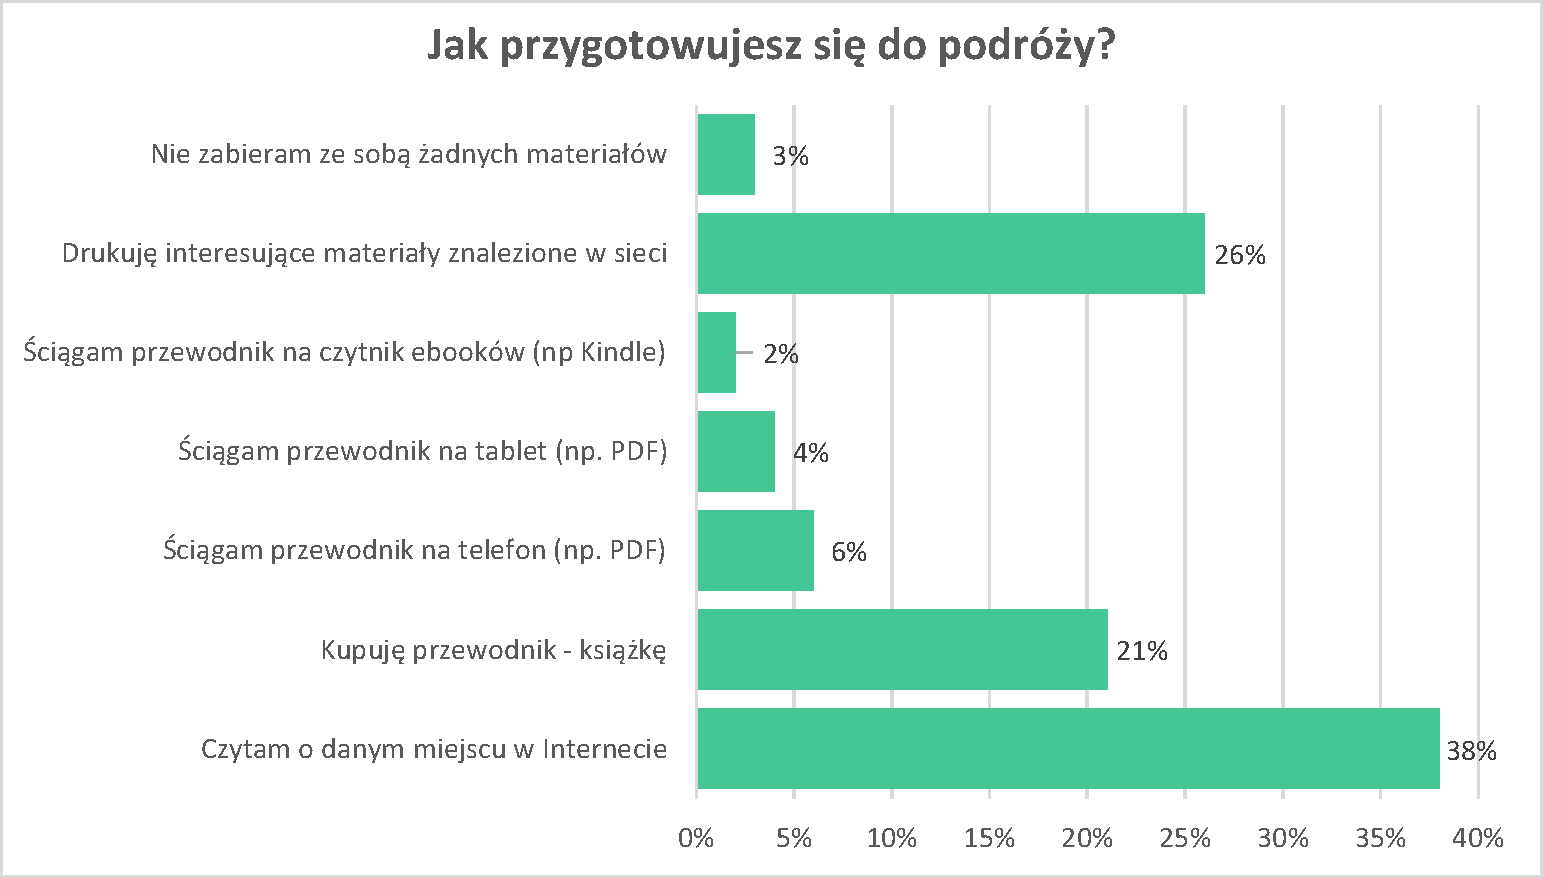
\includegraphics[width=1.0\textwidth]{images/fly4freeAnkieta.pdf}
				\caption{Wyniki ankiety przeprowadzonej wśród użytkowników forum fly4free.pl}
				\label{fig:fly4freeAnkieta}
			\end{figure}
		
	        Praca jest zorganizowana w następujący sposób: 	        
			rozdział \ref{id:cha:wstep} opisuje wprowadzenie do zagadnienia i uzasadnienie podjęcia się takiej tematyki. 
			Rozdział \ref{id:cha:technologia} przedstawia użyte technologie, zarówno w części serwerowej (podrozdział \ref{id:sec:aplikacja_serwerowa}), internetowej (podrozdział \ref{id:sec:web}) jak i mobilnej (podrozdział \ref{id:sec:mobile}). 
			Rozdział \ref{id:cha:specyfikacja_wewnetrzna} zawiera specyfikację wewnętrzną, w tym: opis architektury (podrozdział \ref{id:sec:architektura}), najważniejsze algorytmy (podrozdział \ref{id:sec:algorytmy}) oraz przypadki użycia (podrozdział \ref{id:sec:przypadki_uzycia}). 
			Rozdział \ref{id:cha:specyfikacja_zewnetrzna} zawiera specyfikację zewnętrzną, w tym: wymagania systemowe (podrozdział \ref{id:sec:wymagania}), opis instalacji poszczególnych aplikacji (podrozdział \ref{id:sec:instalacja}) i instrukcję obsługi dla użytkowników końcowych aplikacji mobilnej i internetowej wraz ze zdjęciami systemu (podrozdział \ref{id:sec:instrukcja_obslugi}).
			Rozdział \ref{id:cha:testowanie} opisuje sposób, w jaki projekt był testowany oraz prezentuje wybrane scenariusze testowe. 
			%
			%DOKOŃCZYĆ
			Rozdział \ref{id:cha:wnioski_koncowe} przedstawia wnioski końcowe \ldots				
	
	
	
	\chapter{Technologia}
	\label{id:cha:technologia}
	
	Rozdział opisuje technologie i narzędzia użyte do stworzenia części webowej, serwerowej i mobilnej aplikacji.
	
		\section{Narzędzia}		
			\subsection{Środowisko programistyczne}
				
			Całość projektu została zrealizowana za pomocą Visual Studio 2013. Jest to jedno z popularniejszych środowisk programistycznych, wyprodukowane przez firmę Microsoft. Mimo że nie jest to środowisko bezpłatne, projekt mógł zostać zrealizowany bez ponoszenia kosztów dzięki licencji akademickiej \textit{DreamSpark}. 
			
			Visual Studio 2013 w pełni wspiera rozwijanie oprogramowania w platformie .NET; zarówno rozwiązania mobilne jak i internetowe. Poza tym, dzięki szeregowi dostępnych bibliotek, wspomaga pracę z HTML, LESS oraz JavaScript.
			
			Środowisko to zostało wybrane ze względu na następujące zalety:
			\begin{itemize}
				\item bardzo  dobra obsługa \textit{IntelliSense} dla języka C\#;
				\item wiele pomocnych rozszerzeń, np. \textit{Web Essentials};
				\item wsparcie dla składni języków HTML\footnote{\emph{HyperText Markup Language} -- hipertekstowy język znaczników wykorzystywany do tworzenia stron internetowych.}, CSS\footnote{\emph{Cascading Style Sheets} -- kaskadowe arkusze stylów służące do opisu formy prezentacji strony WWW.} i JavaScript;
				\item wbudowany emulator Windows Phone;
				\item gotowe szablony, które przyspieszają pracę z projektem.
			\end{itemize}
			
			\subsection{System kontroli wersji}
			
			Pomimo że projekt realizowany był indywidualnie, zdecydowano się na wykorzystanie systemu kontroli wersji. Na rynku dostępnych jest wiele takich systemów. Do najpopularniejszych należą: GIT \cite{id:GIT}, Mercurial \cite{id:Mecurial}, SVN \cite{id:SVN}, Bazaar \cite{id:Bazaar} oraz TFS \cite{id:TFS}.
			Podczas projektu zdecydowano się na wykorzystanie systemu GIT. Został on wybrany z wielu powodów. Jest to system rozproszony, więc jego repozytoria są relatywnie małe (np. w porównaniu do SVN). Ponadto GIT oferuje wiele funkcjonalności, które ułatwiają pracę z projektem, m.in. tzw. gałęzie (bardziej elastyczne w porównaniu do gałęzi SVN), etykiety czy lokalną przestrzeń roboczą. Nie bez znaczenia był także fakt, że autorka ma doświadczenie z tym systemem kontroli wersji.

			Repozytorium zostało umieszczone w serwisie Github.com\footnote{Serwis dostępny pod adresem \url{http://github.com}}, który agreguje projekty z całego świata. Portal oferuje przejrzysty interfejs oraz możliwość graficznego przeglądania historii projektu.
		
%		\section{Technologia wykorzystana w części serwerowej}
		\section{Aplikacja serwerowa}
		\label{id:sec:aplikacja_serwerowa}
		Część serwerowa, realizowana jako WebService, wykonana została z wykorzystaniem platformy ASP.NET WebApi 2 \cite{id:WebApi}. Całość opiera się na platformie .NET 4.5 i napisana jest w języku C\#.
		
		W tej części wykorzystano szereg bibliotek. Aby przyspieszyć pracę i zapewnić większe bezpieczeństwo aplikacji, do celów identyfikacji i uwierzytelniania użytkowników została wykorzystana biblioteka AspNet.Identity \cite{id:ASPIdentity}.
		
		Do pracy z kolekcjami wykorzystano bibliotekę LINQ. Jest to zestaw niezwykle przydatnych narzędzi, które ułatwiają pracę z takimi strukturami jak listy, kolejki i inne implementujące interfejs \texttt{IEnumerable}.
		
		Nieodzowna okazała się być biblioteka Newtonsoft.Json \cite{id:NewtonsoftJSON}, która wspomaga formatowanie obiektów na kod JSON\footnote{\emph{JavaScript Object Notation} -- tekstowy format wymiany danych}. Wszystkie akcje zwracające dane zwracają je właśnie w tym formacie. Komunikat w formacie JSON jest literałem obiektu języka JavaScript. Dane przekazywane są jako tablica asocjacyjna a wszystkie dane są zmiennymi.
		
		Jako że WebService działa w innej domenie niż aplikacja użytkownika, niezbędne było dodanie odpowiednich nagłówków HTTP, aby umożliwić zapytania z innej domeny (\emph{Cross Origin Requests}). Bardzo ułatwia to biblioteka Microsoft.AspNet.Cors \cite{id:ASPCors}. Dodaje ona szereg nagłówków wraz z odpowiednio dobranymi parametrami.
		
		WebService komunikuje się z bazą danych, która działa w oparciu o silnik SQL Server 2014 \cite{id:SQLServer}. Komunikacja odbywa się z wykorzystaniem biblioteki Entity Framework \cite{id:EntityFramework}. Jest to biblioteka typu ORM\footnote{\emph{Object-Relational Mapping} -- mapowanie obiektowo-relacyjne. },
		która umożliwia mapowanie wyników pobranych z bazy danych na wcześniej przygotowane modele. Modele te są następnie mapowane na modele przejściowe (\emph{ViewModels}) za pomocą biblioteki AutoMapper \cite{id:Automapper}.
		
%		\section{Technologia wykorzystana w części internetowej} 
		\section{Aplikacja internetowa} 
		\label{id:sec:web}
		Aplikacja internetowa napisana została w modelu \emph{client-side}. Oznacza to, że cała aplikacja interpretowana jest po stronie przeglądarki i nie wymaga specjalistycznego serwera. Aby działała poprawnie, wystarczy dowolny serwer HTTP. Kod został napisany przy użyciu następujących języków: Javascript, HTML i LESS\footnote{\emph{Leaner CSS} -- dynamiczny język arkuszy stylów.}. 
        %		
		Aplikacja stworzona jest w oparciu o platformę AngularJS \cite{keylist}. Jest to zestaw otwartych bibliotek języka JavaScript wspierany przez firmę Google. Umożliwia tworzenie aplikacji internetowych, z których można korzystać bez przeładowania strony (\emph{Single Page Application}). Dane ładowane są w tle dzięki asynchronicznym zapytaniom do WebService realizowanym przez JavaScript.
		
		Zostały również zastosowane poboczne biblioteki. Do najważniejszych zależą:
		
		\begin{description}
			
			\item[LeafletJS] \cite{id:Leaflet} -- 
			umożliwia sprawne dodawanie map do strony. Do wyświetlania map wybrany został silnik OpenStreetMap \cite{id:OpenStreetMaps} ze względu na swoją otwartą licencję.
			\item[jQuery] \cite{id:jQuery} -- 
			jest to zestaw bibliotek pomocniczych dla języka JavaScript. Rozszerza funkcjonalność i upraszcza składnię. W prostszy sposób pozwala na dostęp i manipulację elementami DOM.
			\item[Bootstrap] \cite{id:Bootstrap} -- 
			zestaw bibliotek, który dołączony jest do Twitter Bootstrap. Dostarcza takie moduły jak np. interaktywne wyskakujące okna, animacje zamknięcie i in.
			\item[AngularTranslate.js] \cite{id:AngularTranslate} -- 
			biblioteka rozszerzająca możliwości platformy Angular o implementację wielojęzyczności.  
		
		\end{description}
				
		Za część graficzną aplikacji odpowiada zmodyfikowany przez autorkę szablon AdminLTE \cite{id:AdminLTE} napisany w oparciu o Twitter Bootstrap. Szablon opisany jest językiem LESS, który jest następnie transformowany do CSS.
		
%		\section{Technologia wykorzystana w części mobilnej}
		\section{Aplikacja mobilna}		
		\label{id:sec:mobile}
		Na część mobilną składa się aplikacja dedykowana dla platformy Windows Phone 8.1. Projekt zrealizowany został w modelu Universal Apps, więc cała logika wydzielona jest do osobnego projektu.
		
		Aplikacja wykonana została przy wykorzystaniu platformy .NET, języka C\# oraz XAML. Zaimplementowany został wzorzec architektoniczny MVVM (\emph{Model View ViewModel}, \emph{vide} rozdział \ref{id:subsec:architektura_aplikacji_mobilnej}). W tym celu do projektu dołączona została biblioteka MVVM Light \cite{id:MVVMLight}. 
		
		Aplikacja pobiera dane z WebService i zapisuje je w swojej lokalnej bazie danych. Działa ona dzięki SQLight \cite{id:SQLite}. Do projektu dołączony jest adapter SQLite. Pobrane dane parsowane są do obiektów za pomocą biblioteki Newtonsoft.JSON.


% % % % % % % % % % % % % % % % % % % % % % % % % % % % % % % % % % % % % % % % % % % % % %


	\chapter{Specyfikacja wewnętrzna}
	\label{id:cha:specyfikacja_wewnetrzna}
	
		\section{Architektura}
		\label{id:sec:architektura}
		\begin{figure}		
			\centering
			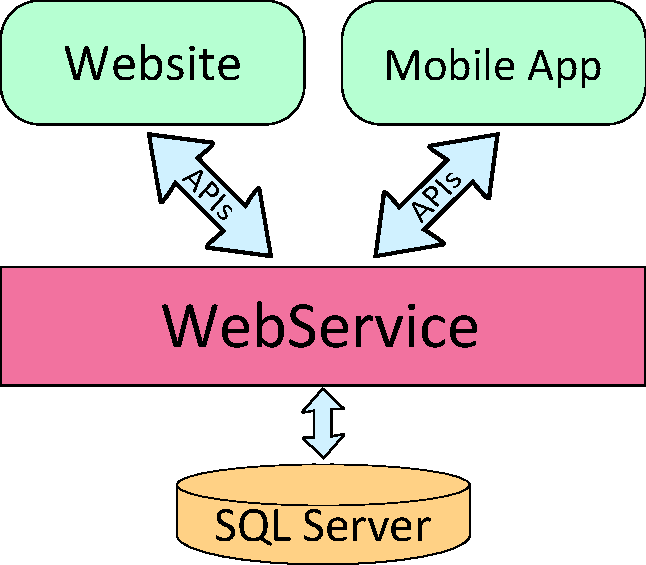
\includegraphics[width=0.5\textwidth]{images/architektura.pdf}
			\caption{Architektura systemu}
			\label{fig:architektura}
		\end{figure}
		
		Na cały system składają się trzy aplikacje: aplikacja mobilna (\emph{Mobile app}), aplikacja internetowa (\emph{Website}) oraz aplikacja serwerowa (\emph{WebService}). Aplikacja serwerowa jest odpowiedzialna za komunikację pomiędzy główną bazą danych a aplikacjami klienckimi. Dostarcza ona API\footnote{Interfejs programistyczny aplikacji (ang. \textit{Application Programming Interface}) -- sposób, w jaki programy komunikują się między sobą.}. Związek pomiędzy tymi aplikacjami przedstawiony jest na rysunku \ref{fig:architektura}. 
			
			\subsection{Architektura aplikacji serwerowej}
			
			Aplikacja serwerowa stworzona jest przy wykorzystaniu platformy ASP.NET WebApi 2 i zgodnie ze wzorcem architektonicznym REST\footnote{\emph{Representational State Transfer}}. Wzorzec ten zakłada kilka warunków:
			
			\begin{description}
				
				\item[Klient-serwer] -- aplikacja powinna składać się z~dwóch odrębnych części: klienta i serwera. Klient nie powinien mieć dostępu do magazynu danych. Serwer z kolei nie powinien zawierać informacji na temat interfejsu użytkownika. I tak też aplikacja serwerowa systemu \appName\ jest jedyną, która ma dostęp do bazy danych. Nie zawiera ona żadnych widoków, a ze światem 				komunikuje się za pomocą zapytań HTTP\footnote{\emph{Hypertext Transfer Protocol} – protokół przesyłania dokumentów hipertekstowych}.
				\item[Bezstanowość] -- każde żądanie HTTP (\emph{request}) wysyłane do serwera jest niezależne od pozostałych. I tak też w aplikacji serwerowej systemu \appName\, za odbiór żądań odpowiada warstwa kontrolera. Każda akcja kontrolera obsługuje jedno żądanie. Akcje są od siebie niezależne.
				\item[Wielowarstwowość] -- klient nie wie, czy jest podłączony bezpośrednio do serwera, czy też otrzymuje informacje przez systemy pośrednie. Dzięki takiej skalowalności, systemy pośrednie mogą zostać wykorzystane, aby zwiększyć wydajność całości. Aplikacja serwerowa systemu \appName\ przyjmuje żądania HTTP a odpowiedź wysyła w formacie JSON. Można więc dołożyć kolejne systemu pośrednie zgodnie z zapotrzebowaniem. 
				\item[Lokalność]\footnote{ang. \textit{cachable}} -- serwer powinien zwracać informację, które z odpowiedzi mogą zostać zapisane w pamięci podręcznej (\emph{cache}) przeglądarki. W przypadku aplikacji serwerowej systemu \appName\ nie jest to zaimplementowane, gdyż żadna z odpowiedzi nie powinna być zapisywana.
				
			\end{description}
			
			\begin{figure}
							\centering
							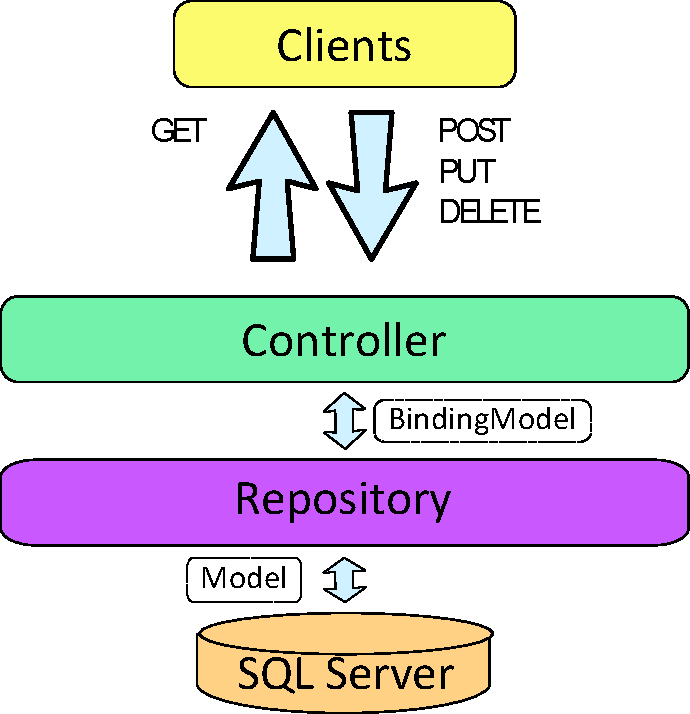
\includegraphics[width=0.5\textwidth]{images/architektura_server.pdf}
							\caption{Architektura aplikacji serwerowej}
							\label{fig:architektura_server}
		    \end{figure}
						
			Wewnętrznie aplikacja składa się z wielu warstw, które komunikują się ze sobą. Każde odebrane zapytanie HTTP jest obsługiwane przez odpowiednią akcję kontrolera. Zapytania realizowane są czterema standardowymi metodami HTTP: \emph{GET}, \emph{POST}, \emph{PUT}, \emph{DELETE}.
			
			Zazwyczaj akcja wymaga interakcji z bazą danych. Kontroler nie komunikuje się z nią jednak bezpośrednio. Zamiast tego składa odpowiednio sparametryzowane zapytanie do warstwy repozytorium. Parametrem może być cyfra (\texttt{Integer}), ciąg znaków (\texttt{String}) lub obiekt typu modelu wiążącego (\emph{Binding Model}). Parametr może być także pusty. 
			
			Repozytorium przetwarza żądanie. Jeżeli parametrem był obiekt typu modelu wiążącego mapuje go na model, a następnie za pomocą \emph{Entity Framework} komunikuje się z bazą danych. Rezultat jest następnie ponownie mapowany na model wiążący i przekazywany do akcji kontrolera. Kontroler zwraca wynik w postaci odpowiedzi HTTP (\emph{HTTP Response}).
			
			Schemat architektury aplikacji serwerowej przedstawiony jest na rysunku \ref{fig:architektura_server}. 			
			
			\subsection{Architektura aplikacji internetowej}		
			
			Aplikacja internetowa została stworzona przy użyciu platformy AngularJS i~w~całości działa bez przeładowania strony (\emph{Single Page Application}). Zawiera główny widok napisany w języku HTML, do którego w zależności od kontekstu załączane są widoki cząstkowe (\emph{partial views}). Z każdym widokiem powiązany jest kontroler. 
			
			Kiedy użytkownik wchodzi w interakcję z aplikacją, jego akcje są wysyłane do odpowiednich akcji kontrolera. Kontroler następnie obsługuje daną operację lub, jeżeli jest ona bardziej skomplikowana, odwołuje się do odpowiedniej metody z warstwy serwisu. Jeżeli wymagane jest pobranie danych z WebService, warstwa serwisu komunikuje się z warstwą repozytorium, która następnie wysyła odpowiednio skonstruowane zapytanie. Otrzymany wynik jest przekazywany z~powrotem do warstwy serwisu, przetwarzany, przekazywany do kontrolera i~wiązany (\emph{Bind}) z~widokiem.								

			Schemat architektury aplikacji internetowej przedstawiony jest na rysunku \ref{fig:architektura_webapp}.	
			
			\begin{figure}
				\centering
				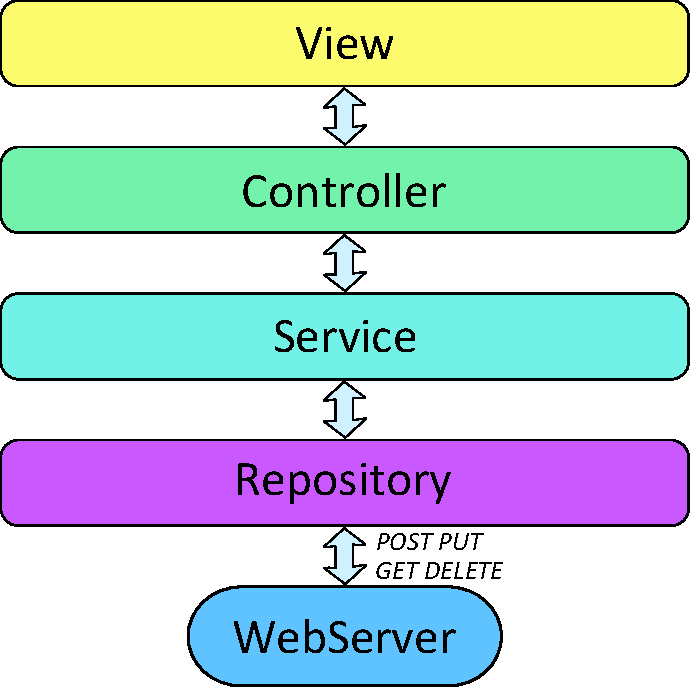
\includegraphics[width=0.5\textwidth]{images/architektura_webapp.pdf}
				\caption{Architektura aplikacji internetowej}
				\label{fig:architektura_webapp}
    		\end{figure}		
			
			\subsection{Architektura aplikacji mobilnej}
			\label{id:subsec:architektura_aplikacji_mobilnej}	
			
			
			Aplikacja mobilna dedykowana jest dla platformy Windows Phone 8.1. Została stworzona przy użyciu wzorca MVVM (\emph{Model View ViewModel}). Wzorzec ten polega na rozdzieleniu warstwy widoku (\emph{View}) od warstwy danych (\emph{Model}). Są one połączone za pomocą warstwy pośredniej (\emph{ViewModel}), która zawiera większą część logiki związanej z prezentacją danych (rys. \ref{fig:mvvmpattern}). Chociaż w początkowym etapie projektu wprowadzenie go wymaga większego nakładu pracy to ma on bardzo wiele korzyści. W przeciwieństwie do utrzymywania kodu w \emph{Code Behind}, gwarantuje niezależność logiki od sposobu wyświetlania danych, brak sztywnych powiązań między widokiem a logiką oraz niezależność kodu od technologii, w której wykonana jest warstwa prezentacji \cite{id:MVVM}.
			
			\begin{figure}
				\centering
				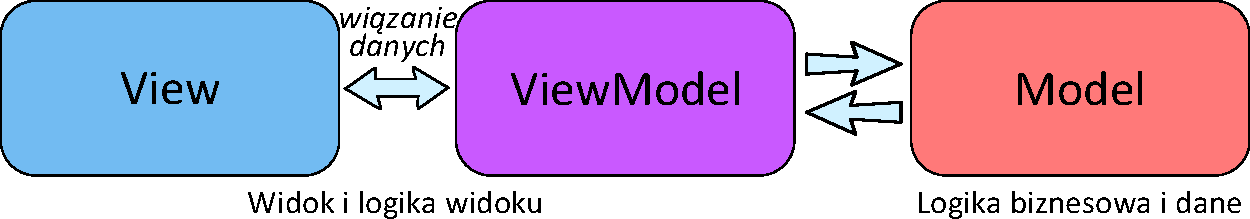
\includegraphics[width=1.0\textwidth]{images/mvvm.pdf}
				\caption{Wzorzec MVVM }
				\label{fig:mvvmpattern}
			\end{figure} 
			
			Program przy pierwszym uruchomieniu łączy się z aplikacją serwerową i~pobiera dane, do których uprawniony jest zalogowany użytkownik. Dane te są zapisywane w lokalnej bazie danych obsługiwanej przez silnik SQLite. 
			
			Użytkownik wchodzi w interakcję z aplikacją przy pomocy zachowań typowych dla obsługi aplikacji mobilnych. Są to gesty takie jak dotknięcie ekranu, dłuższe przytrzymanie ekranu czy posuwisty ruch dłonią po ekranie smartfona. 
			Po stronie aplikacji odbiorcą takich poleceń jest warstwa widoku (\emph{View}). Komunikuje się ona następnie z warstwą pośrednią (\emph{ViewModel}) wprost lub za pomocą konwerterów (\emph{Converter}). Komunikacja odbywa się dzięki wykorzystaniu poleceń (\emph{Commands}. 
			
			Warstwa pośrednia realizuje zadanie zadane przez użytkownika. Jeżeli wymaga to komunikacji z bazą danych, łączy się ona z warstwą repozytorium (\emph{Repository}). Repozytorium operuje na dwóch typach obiektów: na modelach (\emph{Model}) i na modelach wiążących (\emph{Binding model}). Modele odwzorowują schemat bazy danych w postaci obiektów języka C\# i są wykorzystywane w komunikacji z nią. Modele wiążące to modele zmodyfikowane na potrzeby danego zadania.  % \ksremark{To zdanie jest trochę niejasne, warto by je nieco rozwinąć.}
			Są one zmodyfikowane o dodatkowe pola, zbędne pola nie są zaś uwzględnione. Przykładowo, model wiążący wykorzystywany do rejestracji użytkownika stworzony jest na bazie modelu użytkownika. Nie uwzględnia on takich informacji jak ,,Data rejestracji'' bądź ,,Konto Aktywne''. Z drugiej strony jest uzupełniony o takie pole jak ,,Powtórz hasło''.
			
			Za komunikację z aplikacją serwerową odpowiada warstwa serwisów (\emph{Service}), która wysyła do niej odpowiednie zapytania w formacie RESTful. 
			
			Warstwa pośrednia nie wie o istnieniu modeli. Od repozytorium otrzymuje ona jedynie kolekcje modeli wiążących. Finalnie są one przetwarzane i przekazywane do warstwy widoku za pomocą mechanizmu wiązania (\emph{binding}).
			\begin{figure}
				\centering
				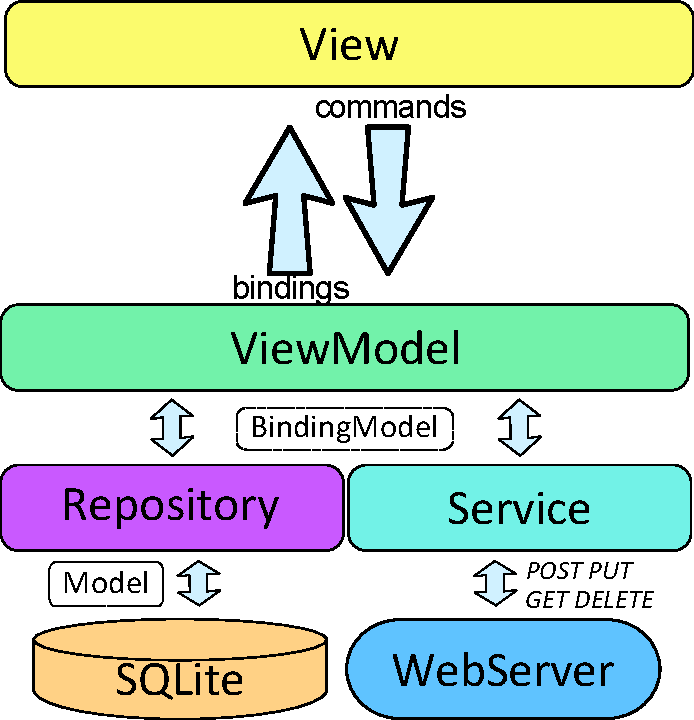
\includegraphics[width=0.5\textwidth]{images/architektura_mobile.pdf}
				\caption{Architektura aplikacji mobilnej}
				\label{fig:architektura_mobile}
			\end{figure}
			
			Schemat architektury aplikacji mobilnej przedstawiony jest na rysunku \ref{fig:architektura_mobile}. 
			
		\section{Najważniejsze algorytmy}
		\label{id:sec:algorytmy}
			\subsection{Wyznaczanie odległości między punktami na mapie}
				
			W celu wyznaczenia odległości pomiędzy miejscami $A$ i $B$ o współrzędnych geograficznych odpowiednio $A(\varphi_a, \lambda_a)$ i $B(\varphi_b, \lambda_b)$ obliczono długość ortodromy łączącej te punkty. Algorytm taki jest dość prosty: należy skonstruować 
			trójkąt sferyczny biorąc jeden z biegunów. Z prawa kosinusów dla trójkąta sferycznego wiemy \cite{id:Mietelski1989Atronomia}:		
		
			\begin{align}
			\cos l & = \cos (\pi/2 - \varphi_a) \cos (\pi/2 - \varphi_b) + \sin (\pi/2 - \varphi_a) \sin (\pi/2 - \varphi_b) \cos (\lambda_a - \lambda_b),
			\end{align}
			gdzie $l$ to kąt ortodromy, wzór można przekształcić
			\begin{align}
			\cos l & = \sin\varphi_a \sin \varphi_b + \cos\varphi_a \cos\varphi_b \cos (\lambda_a - \lambda_b).\label{id:eq:cos:l:2}						
			\end{align}
			Wyznaczenie długości $d$ ortodromy jest proste:
			\begin{align}
			d & =   R_{\earth} l,
			\end{align}
			gdzie $R_{\earth} \approx 6371{,}0\,$km to średni promień Ziemi.
			Uwzględniając równanie \eqref{id:eq:cos:l:2} otrzymujemy
			\begin{align}
		    d & =   R_{\earth} \arccos \left( \sin\varphi_a \sin \varphi_b + \cos\varphi_a \cos\varphi_b \cos (\lambda_a - \lambda_b) \right),\label{id:eq:d}
			\end{align}
			Z tego względu, że dla blisko położonych punktów mogą pojawić się problemy numeryczne (co w dzisiejszych czasach jest już rzadsze), można wzór \eqref{id:eq:d} przekształcić do łatwiejszej obliczeniowo postaci
			\begin{align}
			\label{id:eq:d-haversin}
            d = 2R_{\earth} \arcsin\sqrt{\sin^{2}\left(\frac{\varphi_a - \varphi_b}{2}\right) + \cos\varphi_a\cos\varphi_b\sin^{2}\left(\frac{\lambda_a - \lambda_b}{2}\right) }.
			\end{align}
						
			Oczywiście trzeba pamiętać, że rachunki powyższe nie uwzględniają tego, że Ziemia nie jest kulą, dlatego są obarczone pewnym błędem. Jednakże taki błąd jest dopuszczalny w przypadku aplikacji \appName.
			
		
		Implementacja funkcji w projekcie w języku C\# została przedstawiona na listingu \ref{lst:haversin}. \ksremark{Nie jestem przekonany, czy umieszczać listing w pracy. Tym bardziej, że, implementacja używa funkcji \lstinline!Atan2!, której nie ma we wzorze \ref{id:eq:d-haversin}.}
		
		\begin{lstlisting}[label={lst:haversin},caption=Funkcja obliczająca dystans pomiędzy pozycją użytkownika a punktem na mapie]
		
		public void SetDistance(Geoposition currentPosition)
		{
			const double degreesToRadians = (Math.PI / 180.0);
			const double earthRadius = 6371; // kilometers
			
			// convert latitude and longitude values to radians
			double prevRadLat = _placeLatitude * degreesToRadians;
			double prevRadLong = _placeLongitude * degreesToRadians;
			double currRadLat = currentPosition.Coordinate.Point.Position.Latitude * degreesToRadians;
			double currRadLong = currentPosition.Coordinate.Point.Position.Longitude * degreesToRadians;
			
			// calculate ortodroma
			var exp1 = Math.Pow((Math.Sin((prevRadLat - currRadLat) / 2), 2);
			var exp2 = Math.Cos(prevRadLat)*Math.Cos(currRadLat)*Math.Pow(Math.Sin((prevRadLong-currRadLong)/2) ,2);
			var ortodroma = 2 * earthRadius * Math.Asin(Math.Sqrt(exp1+exp2));
			
			// calculate radian delta between each position.            
			this.Distance = ortodroma * 1000;  // return results as meters
		}
		
		\end{lstlisting}

		%Czy komentarze w kodzie powinny być po polsku?

		\section{Przypadki użycia}
		\label{id:sec:przypadki_uzycia}
		Zarówno aplikacja internetowa jak i mobilna przeznaczona jest dla użytkownika końcowego, jednak ta pierwsza służy użytkownikowi-twórcy a ta druga użytkownikowi-podróżnikowi. Twórca używa aplikacji w następujący sposób: dodaje przewodnik oraz dodaje jego komponenty (podstawowe informacje, miejsca, atrybuty). Następnie może opublikować przewodnik. Twórca ma możliwość także edycji stworzonego przez siebie przewodnika; może edytować jego podstawowe informacje, może edytować, dodawać i usuwać miejsca, atrybuty. 
		
		Użytkownik-podróżnik może pobierać przewodniki a następie je odczytywać i wykorzystywać. W skład tych akcji wchodzi odczyt atrybutów i miejsc a także lokalizowanie położenia tych miejsc i swojego położenia dzięki wbudowanemu w telefon modułowi GPS.  
		 
		Diagram \ref{fig:usecase}) przedstawia najważniejsze przypadki użycia aplikacji klienckich. Pominięta została m.in. funkcja logowania dostępna dla obu aplikacji oraz funkcja rejestracji użytkownika dostępna z poziomu aplikacji mobilnej.			
		
		\begin{figure}		
			\centering
			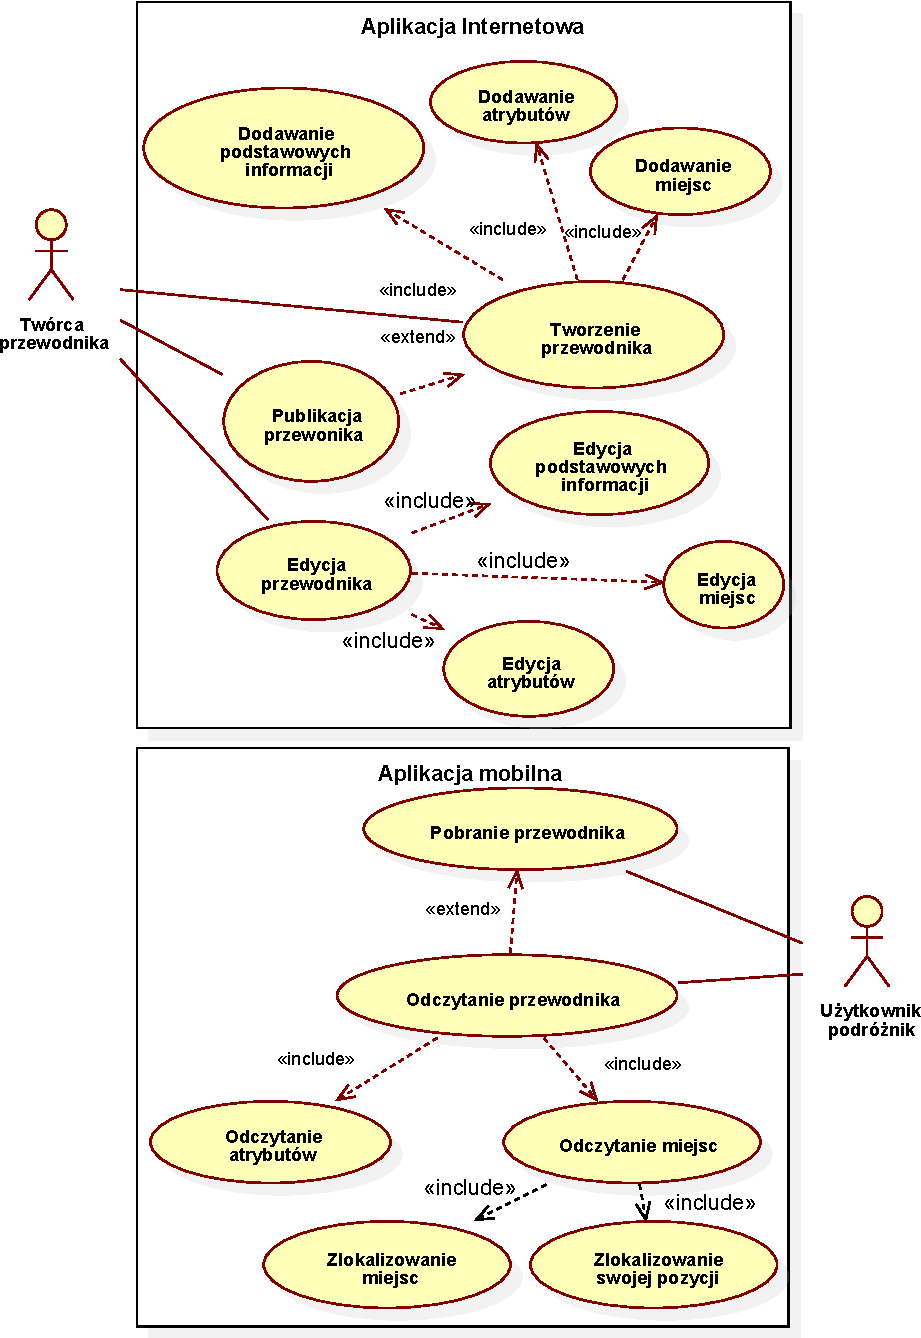
\includegraphics[width=1.0\textwidth]{images/UseCase.pdf}
			\caption{Diagram przypadków użycia}
			\label{fig:usecase}
		\end{figure}
		
		\section{Komponenty}
		\label{id:sec:komponenty}
		Aplikacja serwerowa składa się z kilku komponentów. Do tych głównych należą menedżer użytkowników oraz menedżer przewodników. Menedżer użytkowników odpowiedzialny jest za obsługę logowania oraz rejestracji. Kontroluje on również czy żądanie HTTP jest odpowiednio autoryzowane i czy użytkownik jest uprawniony do wykonania zadanej akcji. Menedżer przewodników służy do zarządzania przewodnikami oraz ich częściami składowymi (miejscami, atrybutami, ikonami etc.). Koordynuje on zarówno proces dodawania, modyfikacji i usuwania ale także pobieranie przewodników, do których użytkownik jest uprawniony. 
		Diagram \ref{fig:component} przedstawia komponenty aplikacji serwerowej. 
		
		
		\begin{figure}		
			\centering
			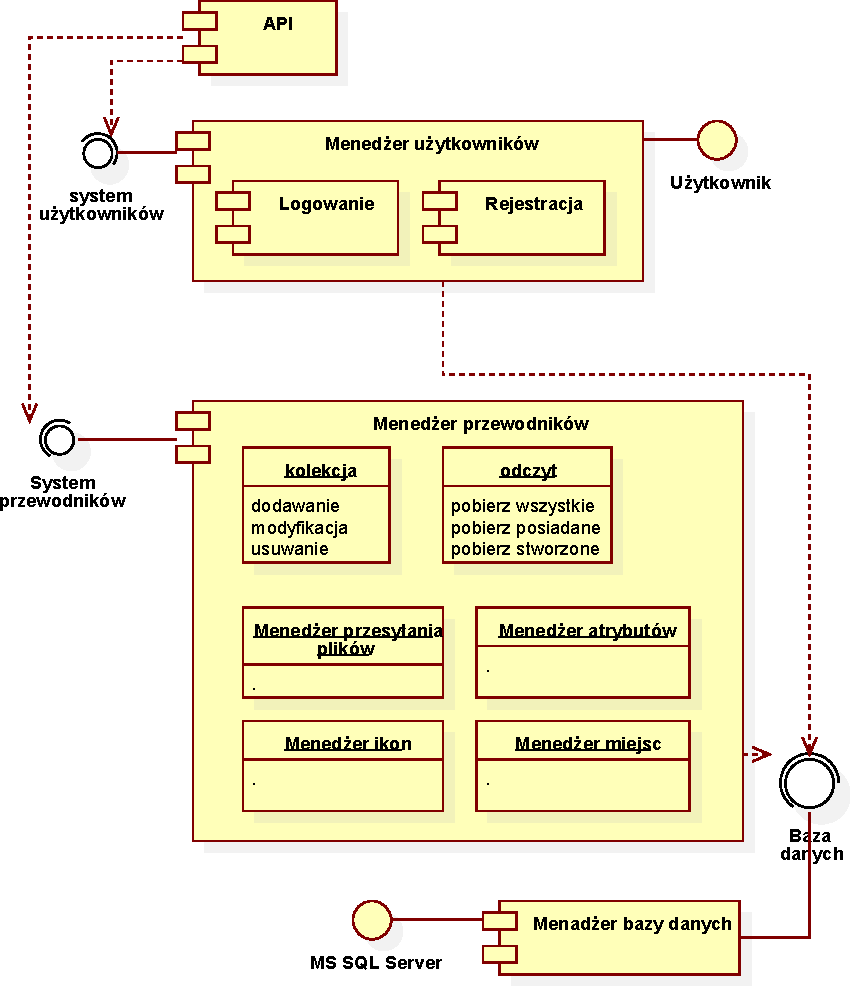
\includegraphics[width=1.0\textwidth]{images/component.pdf}
			\caption{Diagram komponentów}
			\label{fig:component}
		\end{figure}
		
		
	\chapter{Specyfikacja zewnętrzna}
	\label{id:cha:specyfikacja_zewnetrzna}
		\section{Wymagania}
		\label{id:sec:wymagania}
		Aplikacja mobilna zaprojektowana jest z myślą o platformie \emph{Windows Phone 8.1}. Na chwilę obecną nie jest dostępna dla użytkowników systemów \emph{Android} czy \emph{iOS}, jednakże docelowo zostanie dodane wsparcie dla tych platform. Jeżeli użytkownik posiada telefon z systemem \emph{Windows Phone 8}, powinien najpierw zaktualizować swój system. Następnie może pobrać i korzystać z aplikacji. System \emph{Windows Phone 7} nie jest wspierany.
		
		Aplikacja internetowa do poprawnego działania wymaga nowoczesnej przeglądarki z włączoną obsługą JavaScript. Wspierane przeglądarki:
		\begin{itemize}
			\item Google Chrome w wersji 39 lub nowszy;
			\item Mozilla Firefox w wersji 32 lub nowszy;
			\item Opera w wersji 26 lub nowsza;
			\item Internet Explorer 11 lub nowszy.
		\end{itemize}
		
		Aplikacja internetowa działa także na urządzeniach o mniejszych rozdzielczościach takich jak tablety czy telefony.
		
		\section{Instalacja}
		\label{id:sec:instalacja}
		Aplikacja mobilna \appName\ w chwili obecnej zainstalowana może być jedynie na telefonach z odblokowaną opcją deweloperską. Docelowo jednak program zostanie umieszczony w sklepie \emph{Windows Store}, skąd będzie dostępny do pobrania dla użytkowników polsko- i angielskojęzycznych. 
		
		Aplikacja internetowa nie wymaga instalacji. Dostępna jest dla każdego, kto jest podłączony do Internetu, dysponuje kompatybilną przeglądarką internetową i posiada uprawnienia do dodawania nowych przewodników. 
	
	
		\section{Instrukcja obsługi}
		\label{id:sec:instrukcja_obslugi}
		Poniższa sekcja zawiera instrukcję obsługi aplikacji mobilnej i aplikacji internetowej dla użytkowników końcowych. 
		
		\subsection{Instrukcja obsługi aplikacji internetowej}	
		
		\begin{figure}[H]
			
			\begin{subfigure}{1\textwidth}
				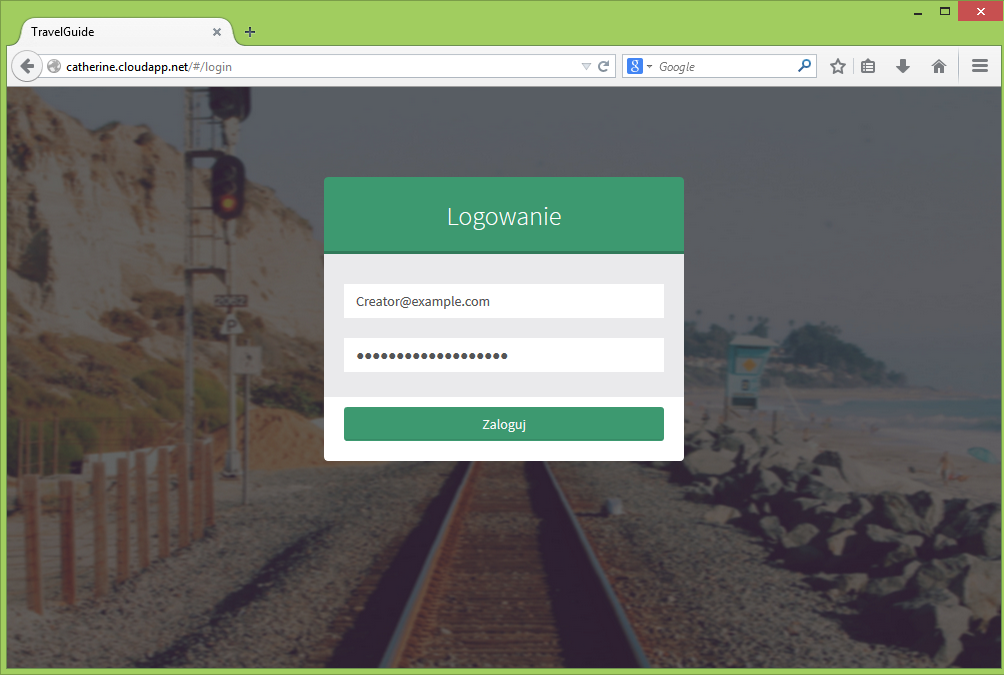
\includegraphics[width=\textwidth]{screenshots/web/1logowanie.png}					
				\caption{\label{subfig:web_login}}
			\end{subfigure}
			\hfill
			\begin{subfigure}{1\textwidth}
				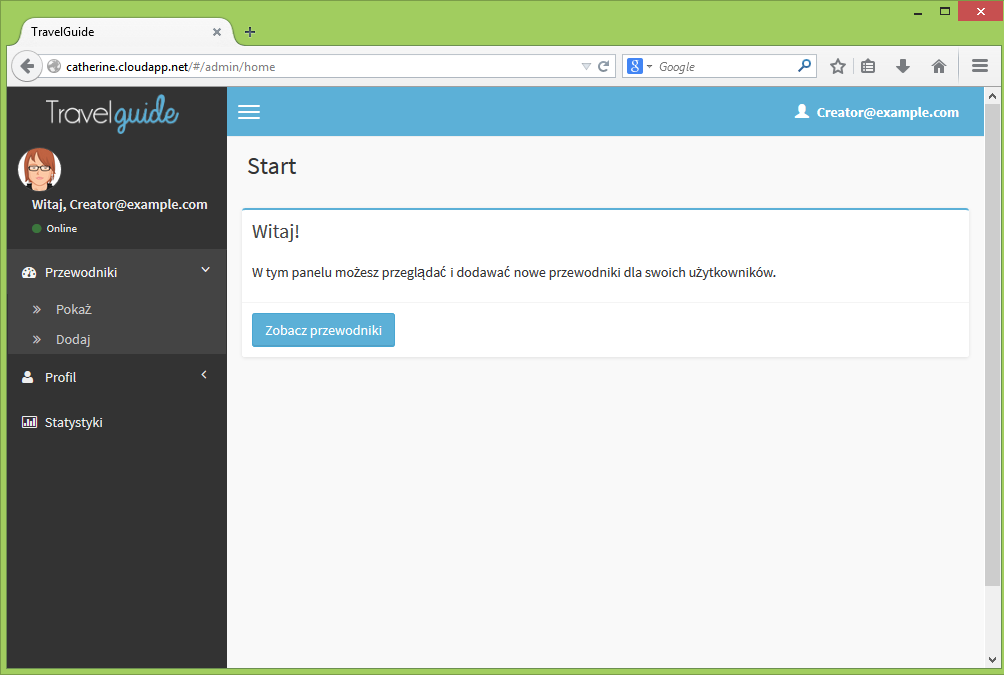
\includegraphics[width=\textwidth]{screenshots/web/2powitanie.png}					
				\caption{\label{subfig:web_welcome}}	
			\end{subfigure}
			
		\end{figure}
		\begin{figure}[H]
			\ContinuedFloat
			
			\begin{subfigure}{1\textwidth}
				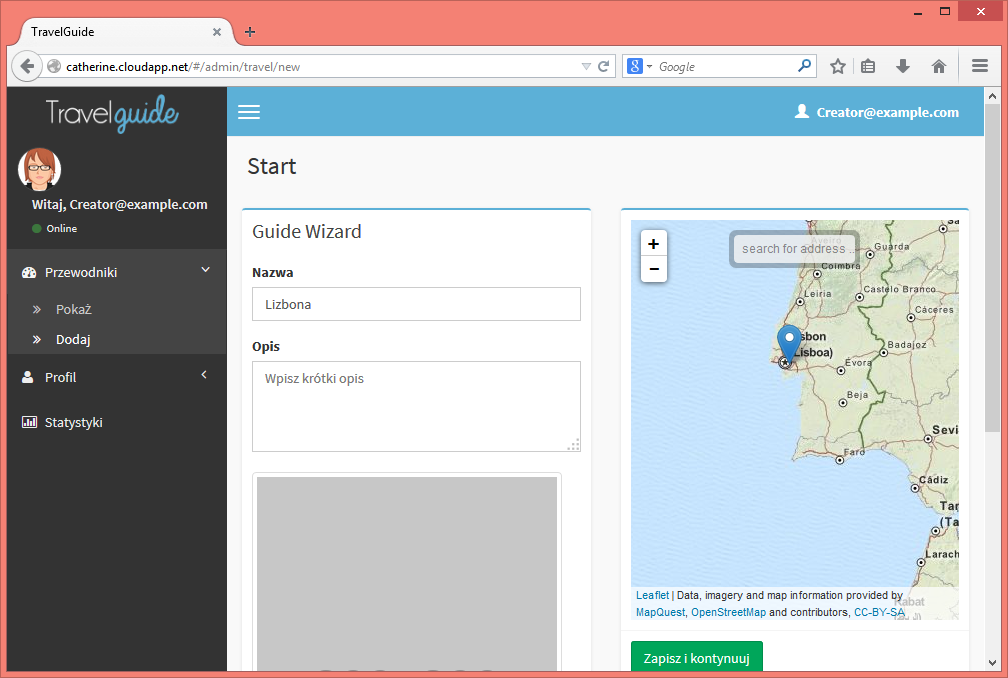
\includegraphics[width=\textwidth]{screenshots/web/3dodawanie.png}					
				\caption{\label{subfig:web_add}	}
			\end{subfigure}
			\hfill			
			\begin{subfigure}{1\textwidth}
				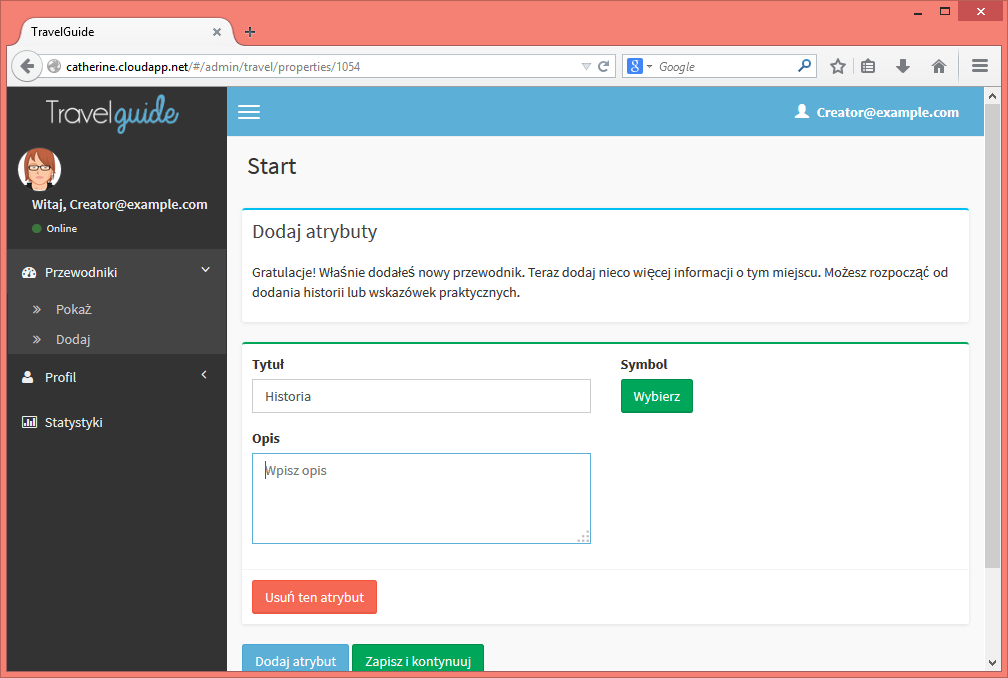
\includegraphics[width=\textwidth]{screenshots/web/4dodawanie2.png}					
				\caption{\label{subfig:web_add2}}
			\end{subfigure}
			
		\end{figure}
		\begin{figure}[H]
			\ContinuedFloat
			
			\begin{subfigure}{1\textwidth}
				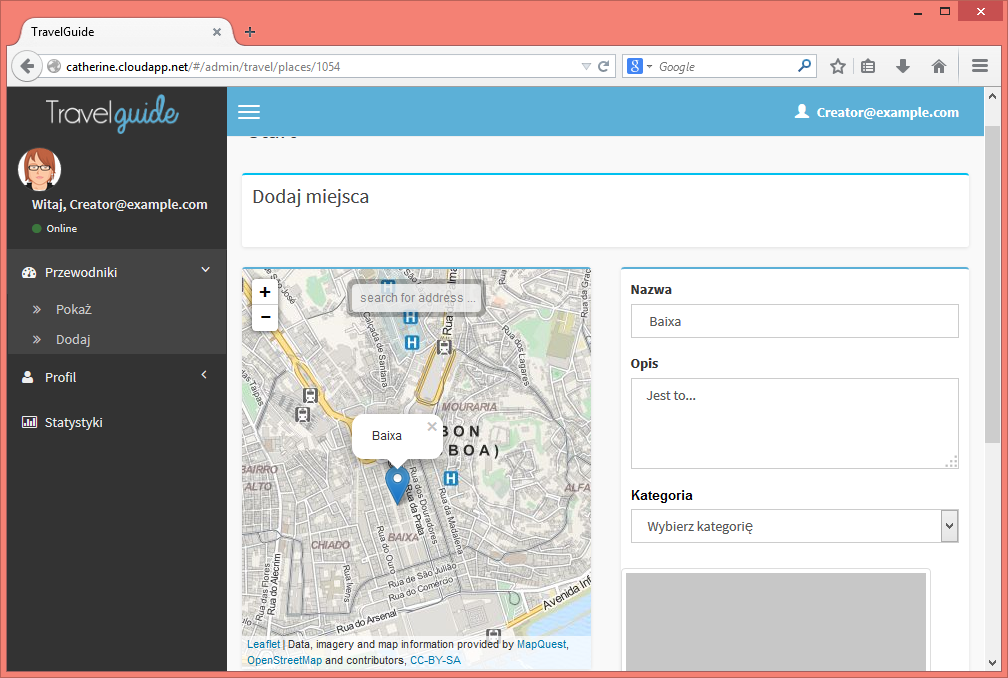
\includegraphics[width=\textwidth]{screenshots/web/5dodawanie3.png}						
				\caption{\label{subfig:web_add3}}
			\end{subfigure}
			\hfill
			\begin{subfigure}{1\textwidth}
				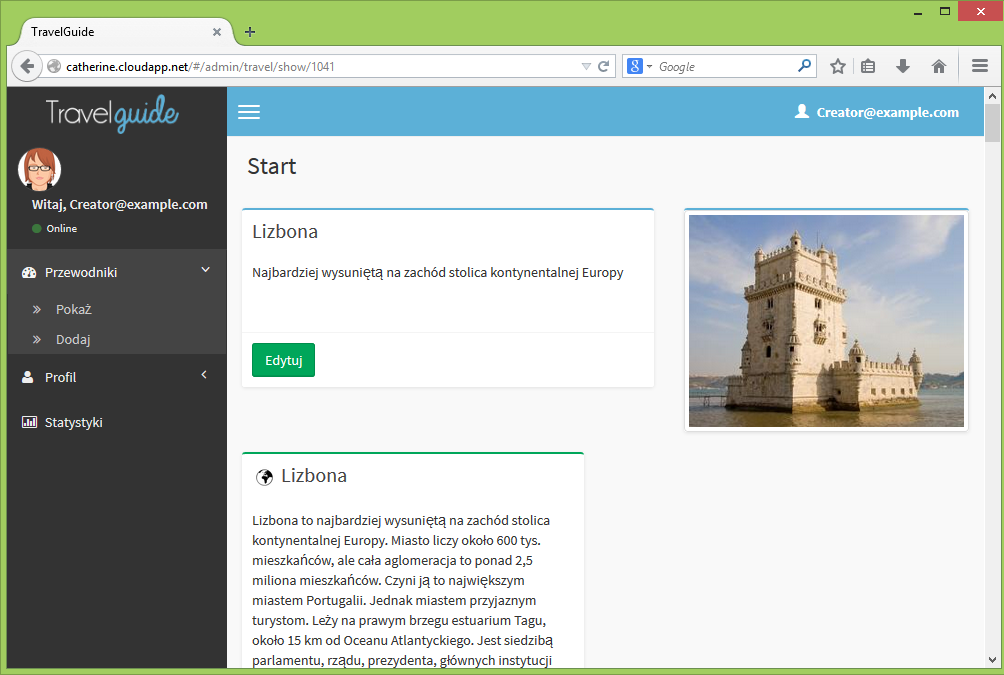
\includegraphics[width=\textwidth]{screenshots/web/6widok.png}
				\caption{\label{subfig:web_view}}	
			\end{subfigure}
			
		\end{figure}
		\begin{figure}[H]
			\ContinuedFloat
			
			\begin{subfigure}{1\textwidth}
				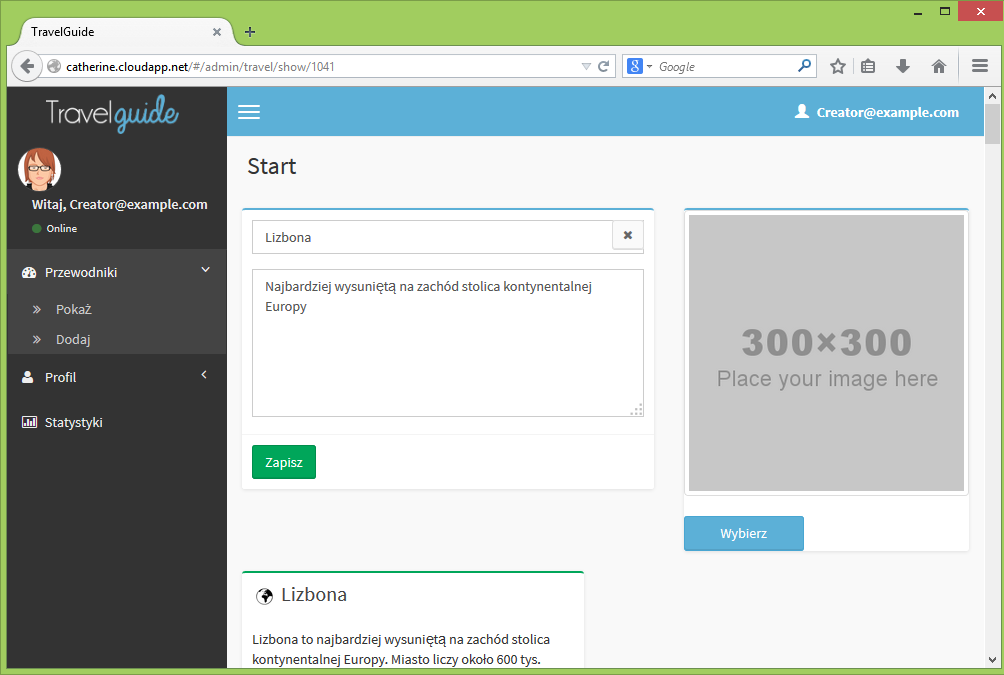
\includegraphics[width=\textwidth]{screenshots/web/7edycja.png}					
				\caption{\label{subfig:web_edit}}
			\end{subfigure}
			\hfill
			\begin{subfigure}{1\textwidth}
				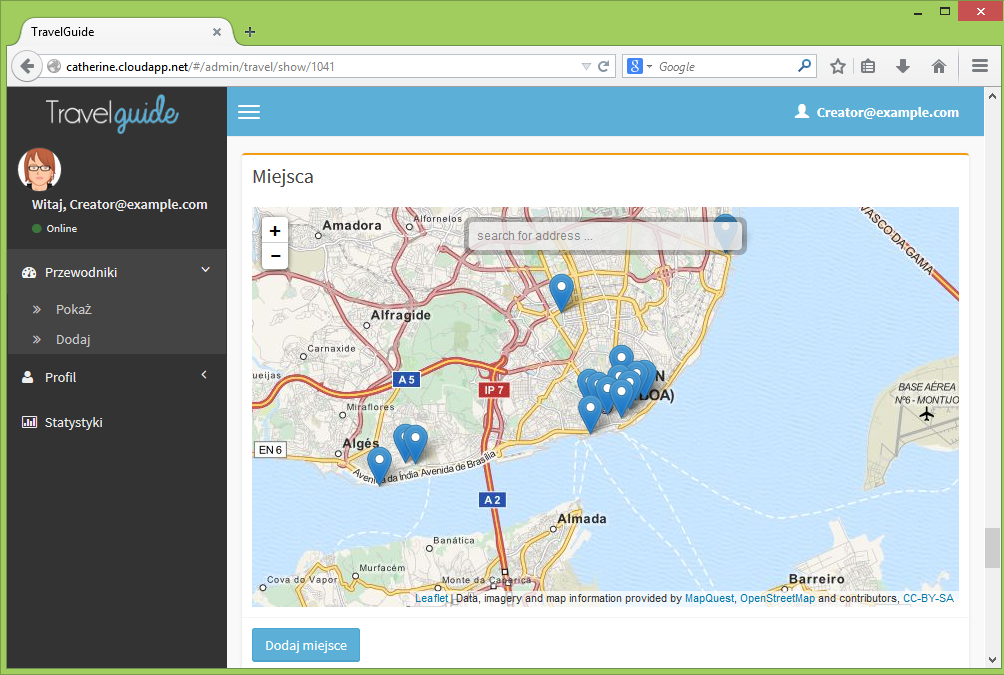
\includegraphics[width=\textwidth]{screenshots/web/8edycja2.png}	
				\caption{\label{subfig:web_edit2}}
			\end{subfigure}
			
		\end{figure}
		\begin{figure}[H]
			\ContinuedFloat
			
			\begin{subfigure}{1\textwidth}
				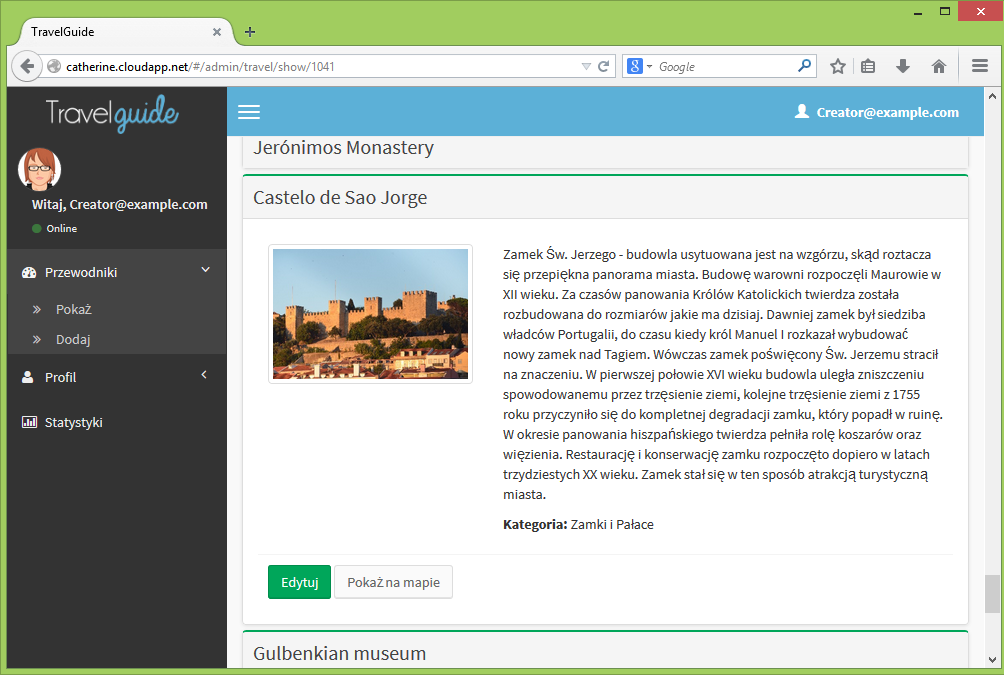
\includegraphics[width=\textwidth]{screenshots/web/9edycja3.png}
				\caption{\label{subfig:web_edit3}}	
			\end{subfigure}
			\hfill
			\begin{subfigure}{1\textwidth}
				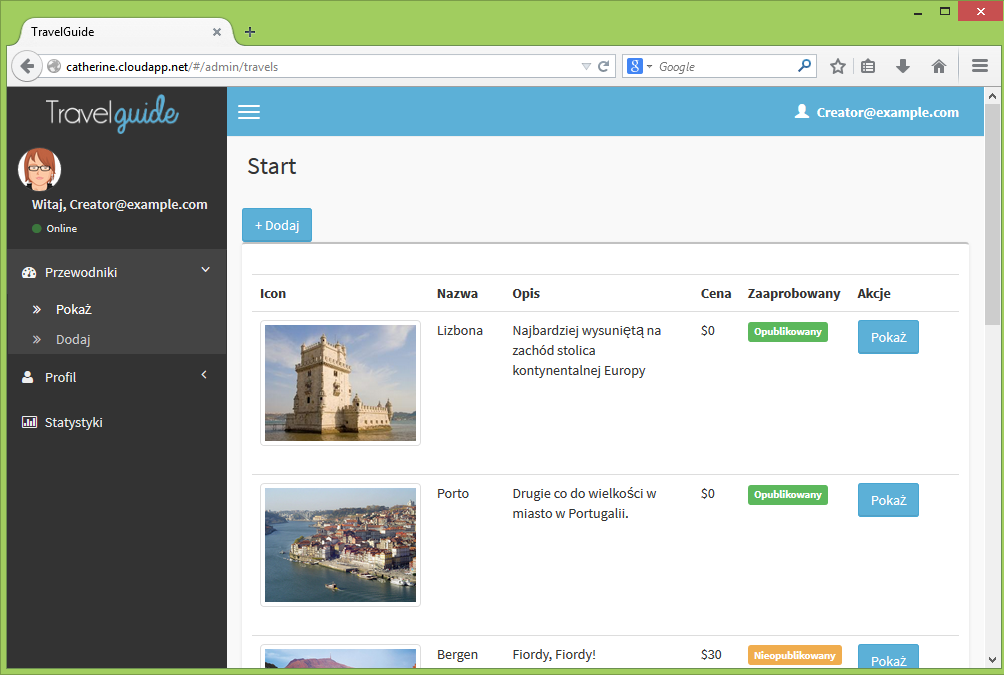
\includegraphics[width=\textwidth]{screenshots/web/10wszystkie.png}
				\caption{\label{subfig:web_all}}	
			\end{subfigure}
		\end{figure}
		
		Niech przykładowym użytkownikiem systemu będzie Marian Pisarz. Marian chce dodać nowy przewodnik o Lizbonie i udostępnić go podróżnikom. Chce również mieć możliwość edycji dodanego przez siebie przewodnika. Poniższy rozdział opisuje sposób dodawania, modyfikacji, przeglądania i publikacji przewodników przez twórców.
		
			\subsubsection{Tworzenie przewodnika}
			
			Marian uruchamia przeglądarkę internetową i wpisuje adres www aplikacji \appName. Przeglądarka przenosi go do ekranu logowanie (rys. \ref{subfig:web_login}). Marian wpisuje swoją nazwę użytkownika i hasło a następnie klika przycisk ,,Zaloguj''. Zostaje przekierowany na stronę powitalną (rys. \ref{subfig:web_welcome}). Następnie wybiera z menu podręcznego opcję ,,Przewodniki'' $\rightarrow$ ,,Dodaj''. Przeglądarka przekierowuje go do kreatora dodawania nowego przewodnika (rys. \ref{subfig:web_add}). 
			
			W kroku pierwszym Marian powinien wymagane pola: wpisać nazwę przewodnika w polu \textit{Nazwa} i opis w polu \textit{Opis}. Następnie, klika na mapę aby zaznaczyć odpowiednie miejsce. Po kliknięciu na mapę pokazuje się na niej niebieski znacznik. Jeżeli Marian popełni błąd, może myszką przeciągnąć znacznik na odpowiednie miejsce. Finalnie, Marian dodaje zdjęcie główne dla przewodnika (okładkę). Może to zrobić na dwa sposoby: przeciągając zdjęcie na szare pole (metoda \textit{Drag and Drop}\footnote{Metoda przeciągnij i upuść}) lub klikając przycisk ,,Dodaj zdjęcie'' i wybierając odpowiedni obrazek z dysku twardego komputera. 
			
			Jeżeli Marian nie wypełni któregoś z pól, przy próbie zapisu otrzyma informację, że dane pole jest wymagane. Jeśli formularz zostanie wypełniony poprawnie, Marian może kontynuować. Zostanie przeniesiony przez swoją przeglądarkę do kroku drugiego kreatora (rys. \ref{subfig:web_add2}). 
			
			W tym etapie kreator tworzenia przewodnika udostępnia możliwość dodania atrybutów, czyli ogólnych informacji o danym miejscu. Marian może dodać takie informacje jak historia, wskazówki dojazdu, ciekawostki, noclegi itp. Na tym etapie atrybuty można dowolnie dodawać i usuwać korzystając z przycisków ,,Dodaj atrybut'' i ,,Usuń ten atrybut''. Każdy atrybut traktowany jest niezależnie i przy każdym atrybucie pola \textit{Tytuł}, \textit{Opis} i \textit{Symbol} są wymagane. Kliknięcie przycisku ,,Wybierz'' pod etykietą \textit{Symbol} powoduje wyświetlenie dodatkowego okna z wyborem możliwych symboli. 
			
			Gdy Marian kończy dodawanie atrybutów naciska przycisk ,,Zapisz i Kontynuuj'' i przechodzi do trzeciego kroku kreatora (rys. \ref{subfig:web_add3}).
			
			W tym etapie należy dodać zestaw interesujących obiektów w danym miejscu. Proces dodawania wygląda następująco: Marian klika na mapie wybierając lokalizację obiektu. Może także skorzystać z wyszukiwarki umieszczonej na górze mapy. Następnie uzupełnia pola \textit{Nazwa}, \textit{Opis} oraz \textit{Kategoria}. Pole \textit{Kategoria} jest polem typu lista rozwijalna i zawiera takie pozycje jak: \textit{Zamki i Pałace}, \textit{Pomniki}, \textit{Kościoły i Cmentarze} itp. Wszystkie pola są wymagane i jest to sprawdzane podczas zapisu.
			Finalnie Marian wybiera obrazek reprezentujący dane miejsce. Proces dodawania obrazka jest taki sam jak w pierwszym kroku kreatora.
			
			Kiedy miejsca zostaną dodane, Marian klika przycisk ,,Zapisz i Kontynuuj''. Przewodnik zostaje zapisany a on zostaje przekierowany na stronę podsumowania (rys \ref{subfig:web_view}).
			
			\subsubsection{Edycja przewodnika}
			
			Strona podsumowania jest jednocześnie stroną, z której możliwa jest edycja przewodnika. Aby edytować opis, nazwę lub zdjęcie danego miejsca, Marian klika zielony przycisk ,,Edytuj''. Statyczna sekcja z opisem zostaje dynamicznie zastąpiona formularzem (rys. \ref{subfig:web_edit}). Tutaj Marian może wprowadzić żądane zmiany. Ponownie jednak żadne pole nie może pozostać puste. Jeżeli na szare pole nie zostanie przeciągnięty żaden obrazek, poprzednia okładka zostaje zachowana. Zmiany można anulować klikając przycisk z symbolem X w prawym, górnym rogu formularza. 
			
			Analogicznie Marian może edytować atrybuty oraz miejsca. Może również usuwać bądź dodawać nowe korzystając z odpowiednich przycisków. Przycisk ,,Dodaj miejsce'' (rys. \ref{subfig:web_edit2}) aktywuje możliwość dodawania markera do mapy oraz dodaje formularz podobny do tego z kroku trzeciego kreatora. 
			
			Przy każdym z miejsc istnieją dwa przyciski: ,,Edytuj'' oraz ,,Pokaż na mapie''. Pierwszy przycisk zastępuje statyczną treść formularzem, podobnie jak ma to miejsce w przypadku informacji ogólnych. Drugi przycisk przenosi użytkownika z powrotem do mapy i oznacza wybrane miejsce chmurką z opisem. 
			
			\subsubsection{Przegląd i publikacja}
		
			Korzystając z menu podręcznego Marian wybiera opcję ,,Przewodniki'' $\rightarrow$ ,,Pokaż''. Zostaje przekierowany do widoku tabeli, w której znajdują się wszystkie dodane przez niego przewodniki (rys. \ref{subfig:web_all}). Oprócz okładki, nazwy i opisu widzi on także status każdego przewodnika. Nieopublikowane przewodniki nie są dostępne do pobrania przez użytkowników aplikacji mobilnej. Aby opublikować swój przewodnik Marian musi nacisnąć przycisk ,,Publikuj''. Od teraz przewodnik może być pobrany na urządzenie mobilne a jego status oznaczony jest zieloną etykietą ,,Opublikowany''. 
		
	\subsection{Instrukcja obsługi aplikacji mobilnej}
	
		\begin{figure}[H]
			
			\begin{subfigure}{0.3\textwidth}
				
\includegraphics[width=\textwidth]{screenshots/mobile/mobile1.png}					
				\caption{\label{subfig:mobile_splash}}
			\end{subfigure}
			\hfill
			\begin{subfigure}{0.3\textwidth}
				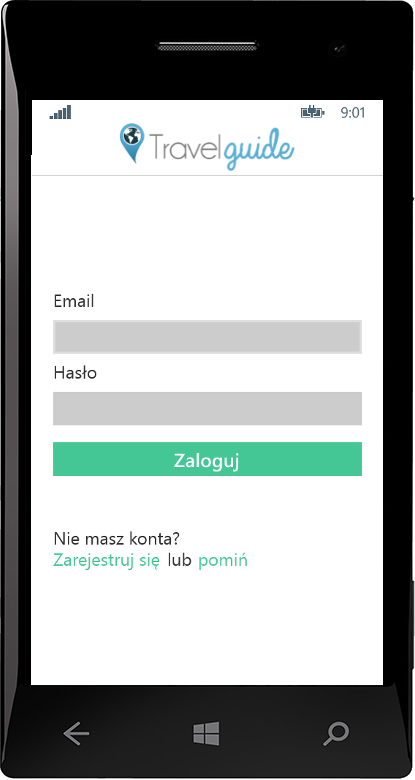
\includegraphics[width=\textwidth]{screenshots/mobile/mobile2.png}					
				\caption{\label{subfig:mobile_login}}	
			\end{subfigure}
			\hfill
			\begin{subfigure}{0.3\textwidth}
				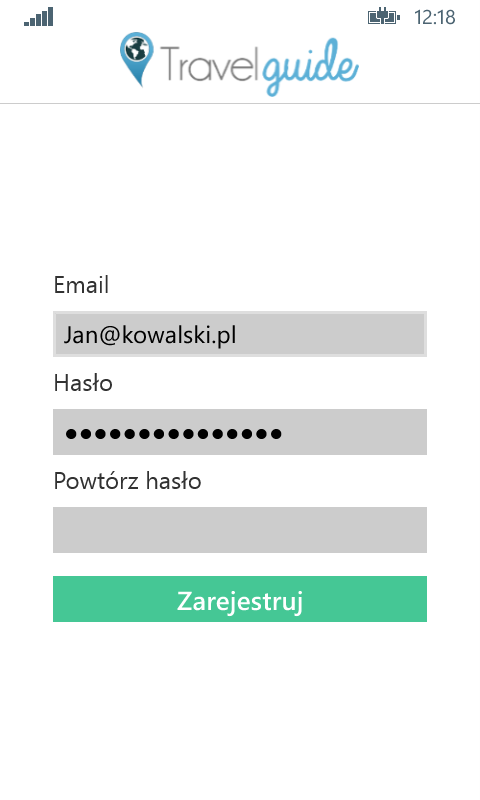
\includegraphics[width=\textwidth]{screenshots/mobile/mobile3.png}					
				\caption{\label{subfig:mobile_register}	}
			\end{subfigure}
			\hfill			
			\begin{subfigure}{0.3\textwidth}
				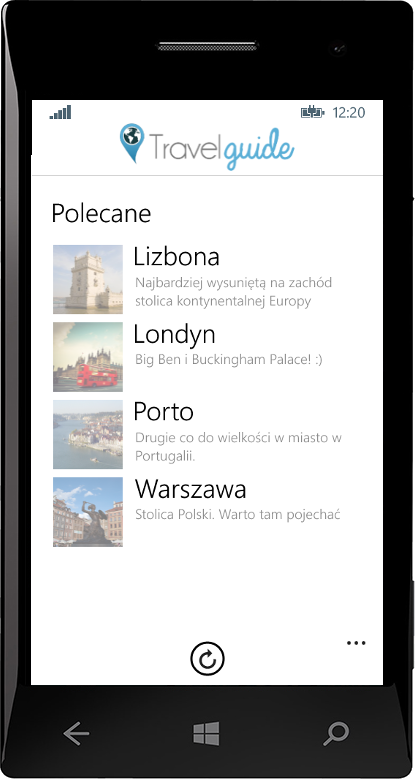
\includegraphics[width=\textwidth]{screenshots/mobile/mobile4.png}					\caption{\label{subfig:mobile_recommended}}
			\end{subfigure}
			\hfill
			\begin{subfigure}{0.3\textwidth}
				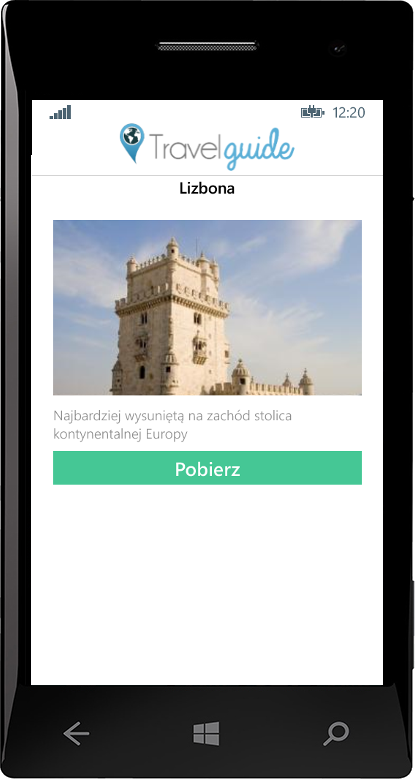
\includegraphics[width=\textwidth]{screenshots/mobile/mobile5.png}						
				\caption{\label{subfig:mobile_buy}}
			\end{subfigure}
			\hfill
			\begin{subfigure}{0.3\textwidth}
				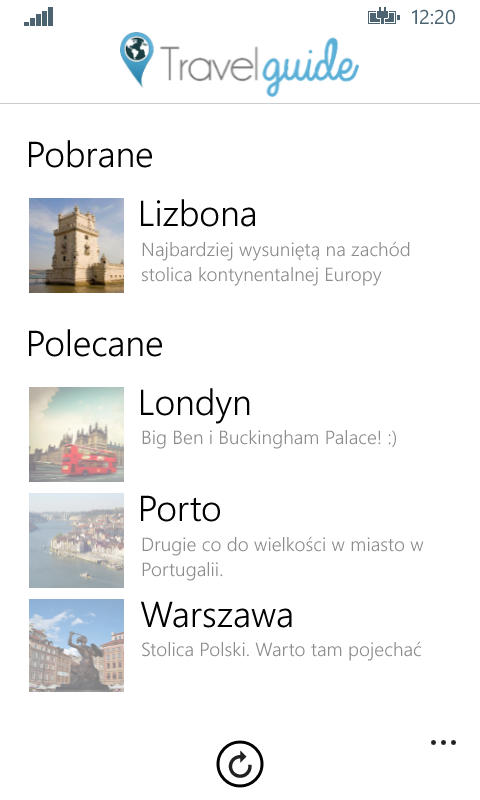
\includegraphics[width=\textwidth]{screenshots/mobile/mobile6.png}
				\caption{\label{subfig:mobile_guides}}	
			\end{subfigure}			
			
		\end{figure}
		\begin{figure}[H]
			\ContinuedFloat
			
			\begin{subfigure}{0.3\textwidth}
				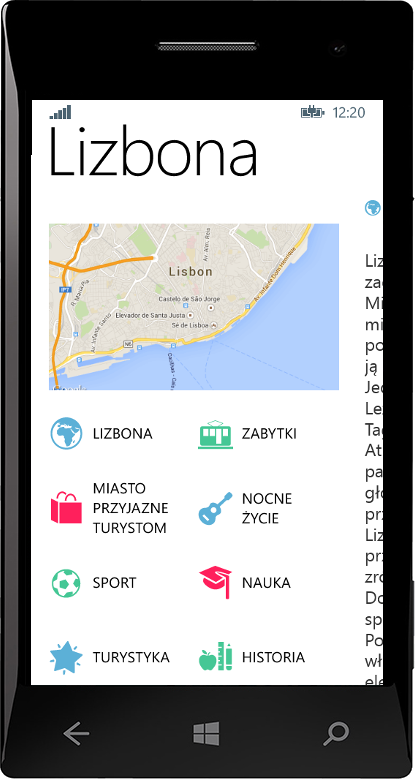
\includegraphics[width=\textwidth]{screenshots/mobile/mobile7.png}	
				\caption{\label{subfig:mobile_guidedetail}}
			\end{subfigure}
			\hfill
			\begin{subfigure}{0.3\textwidth}
				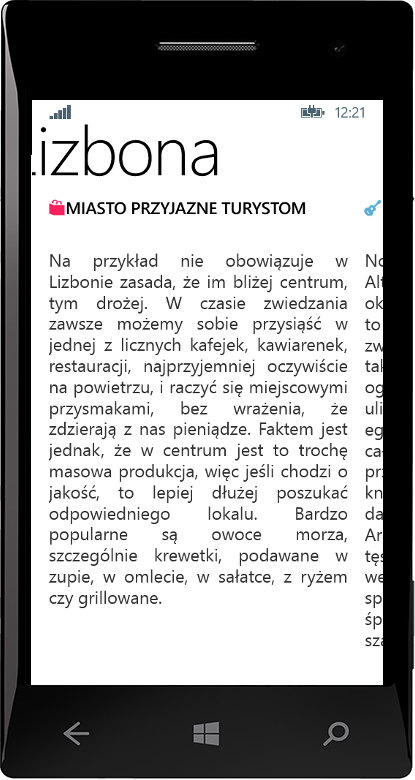
\includegraphics[width=\textwidth]{screenshots/mobile/mobile8.png}	
				\caption{\label{subfig:mobile_guidedetail2}}
			\end{subfigure}
			\hfill
			\begin{subfigure}{0.3\textwidth}
				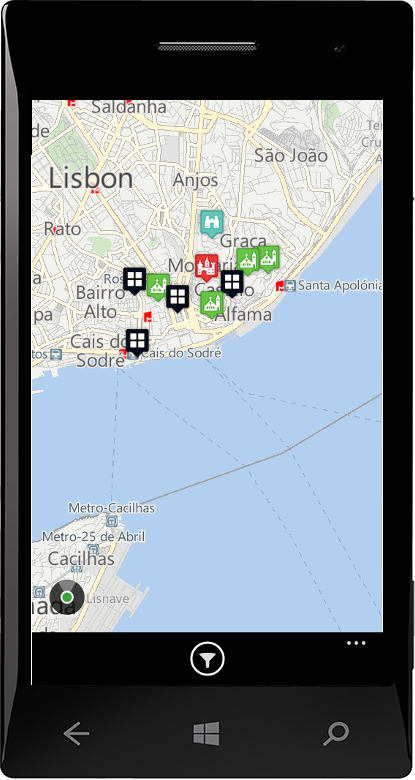
\includegraphics[width=\textwidth]{screenshots/mobile/mobile9.png}
				\caption{\label{subfig:mobile_map}}
			\end{subfigure}
			\hfill
			\begin{subfigure}{0.3\textwidth}
				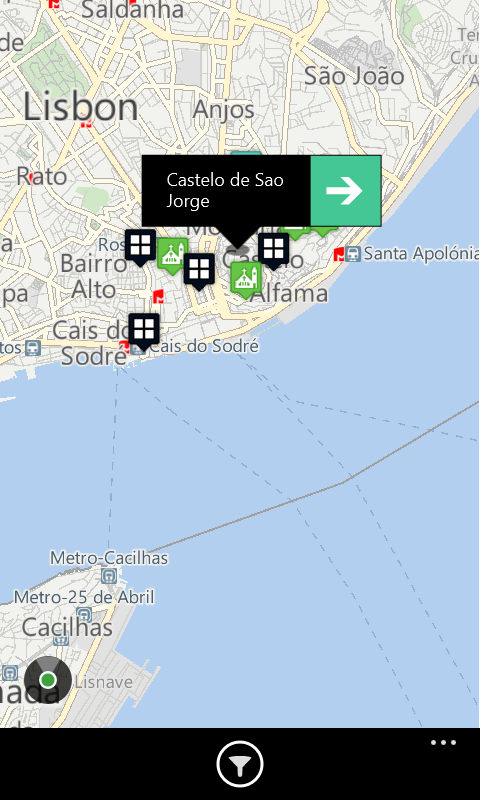
\includegraphics[width=\textwidth]{screenshots/mobile/mobile10.png}
				\caption{\label{subfig:mobile_marker}}		
			\end{subfigure}
			\hfill
			\begin{subfigure}{0.3\textwidth}
				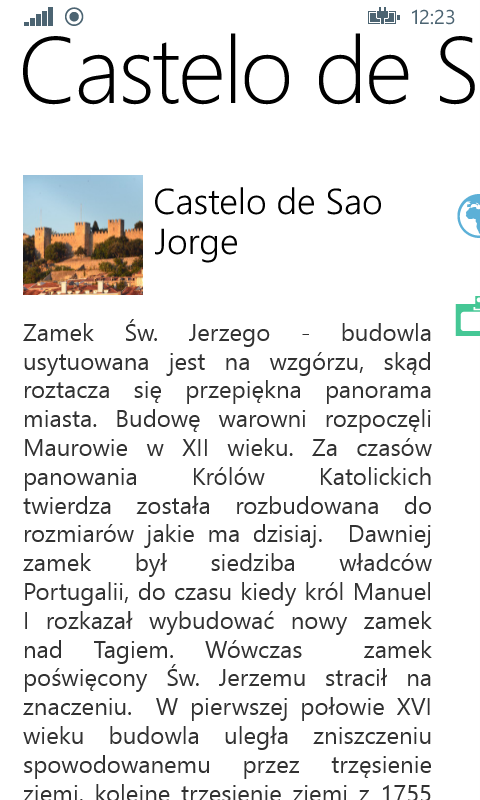
\includegraphics[width=\textwidth]{screenshots/mobile/mobile11.png}	
				\caption{\label{subfig:mobile_place}}	
			\end{subfigure}
			\hfill
			\begin{subfigure}{0.3\textwidth}
				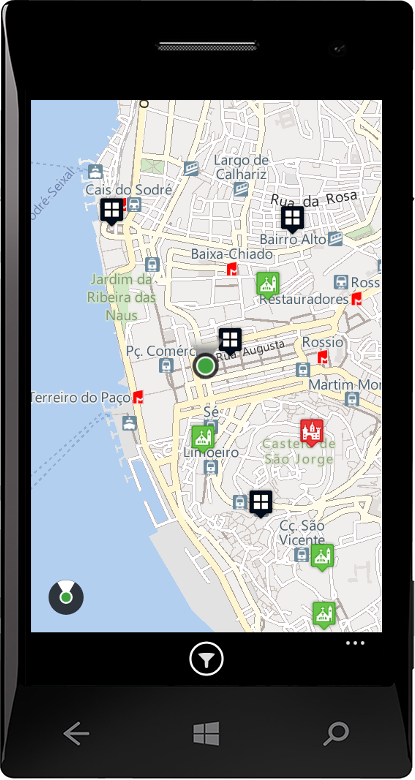
\includegraphics[width=\textwidth]{screenshots/mobile/mobile12.png}	
				\caption{\label{subfig:mobile_navigation}}	
			\end{subfigure}	
			\caption{}
		\end{figure}
		
		Niech przykładowym użytkownikiem systemu będzie Jacek Podróżnik. Jacek wybiera się na krótki urlop do Lizbony i chciałby zaopatrzyć się w aplikację na swój smarfon, która pomoże mu jak najlepiej poznać nowe miejsce.  
		
		Jacek pobiera aplikację z \emph{Windows Store}. Program jest gotowy do użytku zaraz po instalacji. Po włączeniu widoczny jest ekran powitalny z logo (rys.\ref{subfig:mobile_splash}). Chociaż aplikacja może działać w trybie \emph{offline}, podczas pierwszego włączenia wymagane jest połączenie z Internetem. 
		
		Ekran powitalny gaśnie po kilku sekundach i użytkownik jest kierowany do strony logowania (rys. \ref{subfig:mobile_login}). Jeżeli nie posiada on konta może je założyć lub pominąć logowanie i przejść od razu do użytkowania aplikacji. Jacek wybiera opcję rejestracji i jest przenoszony do widoku, w którym musi podać swój adres e-mail oraz hasło z potwierdzeniem (rys. \ref{subfig:mobile_register}). 
		
		Jeżeli podczas rejestracji wystąpią błędy, użytkownik zostanie o tym powiadomiony za pomocą wyskakującego okienka z komunikatem. W przypadku Jacka proces przebiega pomyślnie, i zostaje on przekierowany na stronę z listą polecanych przewodników (\ref{subfig:mobile_recommended}). Tutaj może wybrać interesujący go przewodnik dotykając go na ekranie swojego urządzenia.
		
		Jacek wybiera przewodnik po Lizbonie i zostaje przekierowany do widoku pobierania (rys. \ref{subfig:mobile_buy}). W momencie, kiedy naciska zielony przycisk ,,Pobierz'', aplikacja rozpoczyna pobieranie danych w tle. W tym czasie użytkownik zostaje poinformowany, że aby w pełni używać programu w trybie \emph{offline}, powinien również pobrać mapy dla danego miejsca. Po zamknięciu okienka, Jacek zostaje ponownie przekierowany do widoku przewodników. Tym razem na liście widać świeżo pobrany przewodnik o Lizbonie (rys. \ref{subfig:mobile_guides}). 
		
		Podróżnik dotyka miniaturki Lizbony i przechodzi do właściwej części przewodnika (rys. \ref{subfig:mobile_guidedetail}). W tej sekcji Jacek może poczytać informacje dotyczące miasta (rys. \ref{subfig:mobile_guidedetail2}). Między kolejnymi elementami użytkownik może poruszać się przeciągając palcem po ekranie lub korzystając z przycisków pod mapą. 
		
		Zapoznawszy się z informacjami, Jacek chce dowiedzieć się o ciekawych miejscach w okolicy. Dotyka więc obrazek mapy i zostaje przeniesiony do prawdziwej, interaktywnej mapy z oznaczonymi punktami charakterystycznymi (rys. \ref{subfig:mobile_map}). Po dotknięciu dowolnego z punktów wyświetlona zostaje chmurka z nazwą obiektu i odnośnikiem do szczegółów (rys. \ref{subfig:mobile_marker}). 
		
		Jacek dotyka zielony przycisk ze strzałką i zostaje przeniesiony do strony poświęconej danemu obiektowi (rys. \ref{subfig:mobile_place}). Tu może dowiedzieć się więcej o miejscu oraz zobaczyć miniaturkę zdjęcia.
		
		Powrót do poprzednich widoków odbywa się w sposób standardowy z obsługą systemu \emph{Windows Phone 8.1}; za pomocą fizycznego przycisku wstecz. 		 
	
	\chapter{Testowanie}
	\label{id:cha:testowanie}
	
	Testowanie aplikacji odbywało się w kilku etapach. Na etapie projektowania zostały sprecyzowane wymagania funkcjonalne, jakie każda z aplikacji powinna spełniać. Następnie na podstawie tych wymagań sformułowane zostały scenariusze testowe. W czasie rozwijania kodu, moduły testowane były manualnie. Pod koniec każdego etapu, przeprowadzane były testy akceptacyjne na podstawie scenariuszy testowych. 
	 
	Poniższy rozdział zawiera wybrane scenariusze testowe:

	\begin{itemize}
	\item testowanie aplikacji internetowej:
	   \begin{itemize}
	   \item tworzenie przewodnika (tab. \ref{tab:1})
	   \item tworzenie przewodnika z błędami (tab. \ref{tab:2})
	   \item modyfikacja atrybutu przewodnika (tab. \ref{tab:3})
	   \end{itemize}
	\item testowanie aplikacji mobilnej:
	   \begin{itemize}
	   \item odczytanie informacji o obiekcie turystycznym z przewodnika (tab. \ref{tab:4})
	   \item nawigacja z kompasem  (tab. \ref{tab:5})
	   \item pobranie danych  (tab. \ref{tab:6})
	   \item nieudana próba pobrania danych  (tab. \ref{tab:7})
	   \end{itemize}
	\end{itemize}
	
	\setlength{\tabcolsep}{6pt}
	\renewcommand{\arraystretch}{1.5}
				
			\noindent	
			
		\begin{table}
		\centering
		\caption{Scenariusz testowy dla akcji <<Tworzenie przewodnika>>.}
		\label{tab:1}				    	
			\begin{tabular}{| p {.5\textwidth} | p {.5\textwidth} |}							
				\hline
				\textbf{Cel testu} & Testowanie poprawnego dodawania przewodnika \\
				\hline
				\textbf{Sposób dostępu} & Widok wywołany z poziomu menu ,,Przewodniki'' $\rightarrow$ ,,Dodaj''. Użytkownik powinien posiadać uprawnienia do tworzenia przewodników. \\
				\hline
				\multicolumn{2}{|c|}{\textbf{Scenariusz (kroki testowe)}} \\			
				\hline
				\textbf{Akcja użytkownika} & \textbf{Odpowiedź systemu} \\
				\hline
				
				1. Wpisanie nazwy przewodnika ,,Lizbona'' w pole ,,Nazwa''. & 2. -- \\
				3. Wpisanie opisu ,,Lorem ipsum dolor sit amet'' w pole ,,Opis''. & 4. -- \\
				5. Odnalezienie na mapie miasta Lizbona i kliknięcie w to miejsce. & 6. Wyświetlenie niebieskiego znacznika w miejscu kliknięcia. \\
				7. Przeciągnięcie w szare pole zdjęcia z dysku twardego w formacie png o wymiarach większych niż 500 $\times$ 500 px. & 8. Wyświetlenie wybranego zdjęcia w szarym polu. \\
				9. Kliknięcie przycisku ,,Zapisz i kontynuuj''. & 10. Przekierowanie do strony ,,Dodaj atrybuty'' i informacja o sukcesie. \\
				\hline
			\end{tabular}
  			\end{table}							
  
		\begin{table}
		\centering
		\caption{Scenariusz testowy dla akcji <<Tworzenie przewodnika z błędami>>.}	  
		\label{tab:2}		  	
			\begin{tabular}{| p {.5\textwidth} | p {.5\textwidth} |}					
				\hline
				\textbf{Cel testu} & Testowanie walidacji pól podczas dodawania przewodnika \\
				\hline
				\textbf{Sposób dostępu} & Widok wywołany z poziomu menu ,,Przewodniki'' $\rightarrow$ ,,Dodaj''. Użytkownik powinien posiadać uprawnienia do tworzenia przewodników. \\
				\hline
				\multicolumn{2}{|c|}{\textbf{Scenariusz (kroki testowe)}} \\			
				\hline
				\textbf{Akcja użytkownika} & \textbf{Odpowiedź systemu} \\
				\hline
				
				1. Pozostawienie pole ,,Nazwa'' i pole ,,Opis'' pustym. & 2. -- \\
				3. Przeciągnięcie w szare pole zdjęcia z dysku twardego w formacie png o wymiarach większych niż 500x500 px. & 4. Wyświetlenie wybranego zdjęcia w szarym polu. \\
				5. Kliknięcie przycisku ,,Zapisz i kontynuuj''. & 6. Wyświetlenie informacji błędach: ,,Nazwa nie może być pusta'', ,,Opis nie może być pusty'', ,,Proszę wybrać miejsce''. \\
				\hline
			\end{tabular}
			\end{table}
		
		\begin{table}
		\centering
		\caption{Scenariusz testowy dla akcji <<Modyfikacja atrybutu przewodnika>>.}
		\label{tab:3}		
			\begin{tabular}{| p {.5\textwidth} | p {.5\textwidth} |}					
				\hline
				\textbf{Cel testu} & Testowanie edycji atrybutu przewodnika \\
				\hline
				\textbf{Sposób dostępu} & Widok wywołany z poziomu menu ,,Przewodniki'' $\rightarrow$ ,,Pokaż''. Wybrany przewodnik: ,,Lizbona''. Użytkownik powinien posiadać uprawnienia do tworzenia przewodników i być twórcą przewodnika ,,Lizbona''. \\
				\hline
				\multicolumn{2}{|c|}{\textbf{Scenariusz (kroki testowe)}} \\			
				\hline
				\textbf{Akcja użytkownika} & \textbf{Odpowiedź systemu} \\
				\hline
				1. Odnalezienie atrybutu ,,Historia'' i kliknięcie ,,Edytuj''. & 2. Podmiana tekstów wybranego atrybutu na pola tekstowe. Podmiana obrazku symbolu na przycisk. \\
				3. Zmiana tytułu atrybutu na ,,Lizboński renesans''. Dodanie ,,Lorem ipsum'' do opisu. & 4. --\\
				5. Kliknięcie przycisku z ikoną symbolu. & 6. Wyświetlenie wyskakującego okna z dostępnymi symbolami. \\
				7. Wybranie symbolu z 3 rzędu, 2 kolumny. & 8. Wyświetlenie nowo wybranego symbolu w miejscu starego. \\
				9. Kliknięcie przycisku ,,Zapisz'' & 10. Podmiana pól tekstowych i przycisku symbolu na statyczny tekst z uwzględnieniem zmian. \\				
				\hline
			\end{tabular}
		\end{table}
	
		\begin{table}
		\centering
		\caption{Scenariusz testowy dla akcji <<Odczytanie informacji o obiekcie turystycznym z przewodnika>>.}
		\label{tab:4}		    	
			\begin{tabular}{| p {.5\textwidth} | p {.5\textwidth} |}							
				\hline
				\textbf{Cel testu} & Testowanie poprawnego odczytu informacji o danym miejscu \\
				\hline
				\textbf{Sposób dostępu} & Widok wywołany poprzez włączenie aplikacji. Użytkownik powinien być zalogowany i mieć przewodnik ,,Lizbona'' już pobrany na swój telefon. \\
				\hline
				\multicolumn{2}{|c|}{\textbf{Scenariusz (kroki testowe)}} \\			
				\hline
				\textbf{Akcja użytkownika} & \textbf{Odpowiedź systemu} \\
				\hline
				1. Wybranie listy pobranych przewodników pozycję ,,Lizbona''. & 2 Wyświetlenie widoku przewodnika. \\
				3. Dotknięcie obrazku mapy. & 4. Wyświetlenie widoku mapy wraz z markerami miejsc. \\
				5. Wybranie markera opisanego jako ,,Castelo de Sao Jorge''. & 6. Wyświetlenie chmurki z nazwą miejsca. \\
				7. Dotknięcie przycisku z białą strzałką na zielonym tle. & 8. Wyświetlenie widoku miejsca wraz z jego opisem. \\
				\hline
			\end{tabular}
		\end{table}
		
		\begin{table}
		\centering
		\caption{Scenariusz testowy dla akcji <<Nawigacja z kompasem>>.}
		\label{tab:5}
      		\begin{tabular}{| p {.5\textwidth} | p {.5\textwidth} |}							
				\hline
				\textbf{Cel testu} & Testowanie poprawnego działania nawigacji z kompasem \\
				\hline
				\textbf{Sposób dostępu} & Widok wywołany poprzez wybranie z pobranych przewodników pozycji ,,Lizbona'' i przejście do mapy. Użytkownik powinien być zalogowany i mieć ten przewodnik już pobrany na swój telefon. GPS powinien być aktywny. \\
				\hline
				\multicolumn{2}{|c|}{\textbf{Scenariusz (kroki testowe)}} \\			
				\hline
				\textbf{Akcja użytkownika} & \textbf{Odpowiedź systemu} \\
				\hline
				1. Dotknięcie zielonego markera GPS w prawym, dolnym roku. & 2. Wycentrowanie mapy do aktualnej pozycji użytkownika. \\
				3. Ponowne dotknięcie markera GPS. & 4. Wyświetlenie szarego pola możliwych pozycji i obrót mapy tak, aby północ wskazywała faktyczną północ telefonu. \\
				5. Obrót telefonem & 6. Obrót mapy zgodnie z obrotem telefonu. \\
				\hline
			\end{tabular}
		\end{table}

		\begin{table}
		\centering
		\caption{Scenariusz testowy dla akcji <<Pobieranie danych>>.}
		\label{tab:6}
			\begin{tabular}{| p {.5\textwidth} | p {.5\textwidth} |}							
				\hline
				\textbf{Cel testu} & Testowanie poprawnego działania pobierania danych \\
				\hline
				\textbf{Sposób dostępu} & Widok wywołany poprzez włączenie aplikacji. Użytkownik powinien być zalogowany. Transfer danych powinien być aktywny. \\
				\hline
				\multicolumn{2}{|c|}{\textbf{Scenariusz (kroki testowe)}} \\			
				\hline
				\textbf{Akcja użytkownika} & \textbf{Odpowiedź systemu} \\
				\hline
				1. Dotknięcie ikony ,,odśwież'' znajdującej się na pasku aplikacji. & 2. Wyświetlenie kółka postępu. \\
				3. Oczekiwanie & 4. Wyświetlenie pobranych przewodników w dwóch kategoriach: ,,Pobrane'' i ,,Polecane'' \\
				\hline
			\end{tabular}
		\end{table}
			
		\begin{table}
		\centering
		\caption{Scenariusz testowy dla akcji <<Nieudana próba pobrania danych>>.}
		\label{tab:7}
			\begin{tabular}{| p {.5\textwidth} | p {.5\textwidth} |}							
				\hline
				\textbf{Cel testu} & Testowanie obsługi błędów podczas pobierania danych \\
				\hline
				\textbf{Sposób dostępu} & Widok wywołany poprzez włączenie aplikacji. Użytkownik powinien być zalogowany. Transfer danych powinien być wyłączony. \\
				\hline
				\multicolumn{2}{|c|}{\textbf{Scenariusz (kroki testowe)}} \\			
				\hline
				\textbf{Akcja użytkownika} & \textbf{Odpowiedź systemu} \\
				\hline
				1. Dotknięcie ikony ,,odśwież'' znajdującej się na pasku aplikacji. & 2. Wyświetlenie kółka postępu. \\
				3. Oczekiwanie & 4. Wyświetlenie komunikatu o braku połączeniu z Internetem. Wyświetlenie poprzednich pozycji na listach. \\
				\hline
			\end{tabular}
		\end{table}
	
	\chapter{Wnioski końcowe}
	\label{id:cha:wnioski_koncowe}
	
	%​We wnioskach końcowych można opisać:
	%* ​uzyskane wyniki w świetle postawionego celu
	%* kierunki ewentualnych dalszych prac (rozbudowa funkcjonalności)
	%* problemy napotkane w czasie pracy
	
	\section{Kierunek dalszych prac}
	
	Projekt przebiegł pomyślnie i udało się osiągnąć założone cele. Powstała w pełni funkcjonalna aplikacja mobilna, która gotowa jest do użytku przez użytkowników końcowych. Aplikacja internetowa wymaga jeszcze kilku dodatkowych funkcjonalności przed wdrożeniem jej do publicznego użytku. Są to: funkcja edycji konta użytkownika, funkcja przywracania i zmiany hasła, rola administratora i możliwość zarządzania użytkownikami, tworzenie nowych kont dla twórców. W przyszłości warto byłoby wdrożyć także panel administracyjny dla użytkowników-podróżników, gdzie mieliby oni wgląd do pobranych przez siebie przewodników oraz mogliby pobierać kolejne. Jedną z dodatkowych możliwości rozwoju jest umożliwienie podróżnikom tworzenie i publikowanie własnych przewodników.
	
	Aplikacja mobilna także posiada bardzo wiele perspektyw rozwoju. W pierwszej kolejności warto byłoby stworzyć wersję dla systemów iOS oraz Android, gdyż są one bardziej popularne niż platforma Windows Phone. Ponadto, do aplikacji można wdrożyć funkcję wirtualnego przewodnika. Polegałaby ona na tym, że użytkownik wybierałby miejsca, które chce odwiedzić a aplikacja obliczałaby optymalną drogę pomiędzy nimi. Następnie tryb mapy przełączałby się w tryb nawigacji i użytkownik byłby prowadzony do kolejnych punktów i informowany na bieżąco o tym, co znajduje się wokół niego. Można by tu także pomyśleć o wykorzystaniu rozszerzonej rzeczywistości. 
	
	\section{Napotkane problemy}
	
	Podczas realizacji projektu pojawiło się wiele nieoczekiwanych problemów. Po pierwszych testach aplikacji mobilnej okazało się, że pobieranie danych jest bardzo niewydajne. Algorytmy zostały więc zoptymalizowane i pobieranie znacznie przyśpieszyło. Problematyczne było także pierwsze zetknięcie z Bing Maps API. Dostosowanie zachowania mapy wymagało więcej czasu niż zakładano. 
	
	Również aplikacja serwerowa przeniosła kilka niespodziewanych problemów. Pierwotnie zaczęła być ona rozwijana w oparciu o platformę Groovy on Grails\cite{id:GroovyOnGrails}, szybko jednak została przeniesiona do technologii .NET. Zanim zdecydowano się na wykorzystanie platformy Web API poczyniono podejście do technologii WCF\cite{id:WCF}. Web Api zostało wybrane, gdyż jest ono znacznie prostsze niż WCF, nowsze lecz dobrze udokumentowane.
	
	Początkowo problematyczne było odpowiednie podzielenie solucji na projekty, co skutkowało wielokrotną refaktoryzacją kodu. Finalnie projekt nabrał prawidłowych kształtów zgodnych ze wzorcami projektowymi opisanymi w sekcji \ref{id:sec:architektura}. 
	
	Niespodziewanym problemem, który ujawnił się dopiero po instalacji aplikacji na zdalnym serwerze, była blokada zapytań pochodzącej z innej domeny. Problem oraz jego rozwiązanie zostały szczegółowo opisane w sekcji \ref{id:sec:aplikacja_serwerowa}.
	
	Aplikacja internetowa nie od razu została napisana przy użyciu platformy Angular. Przeprowadzono eksperymenty z EmberJS\cite{id:Ember} oraz BackboneJS\cite{id:Backbone}. EmberJS okazał się być zbyt młodą biblioteką, której zabrakło wsparcia dla serwisów Web API; Backbone okazał się zbyt ciężki oraz dość trudny w skonfigurowaniu w środowisku IIS. Finalnie wybrano więc AngularJS. Jako, że ta biblioteka była nowością dla autorki, sporo czasu zostało poświęcone na naukę i zrozumienie zasady działania platformy. Problematyczne było pierwsze podejście do konfiguracji, jednakże dzięki bogatym zasobom w Internecie udało się ten problem sprawnie pokonać. 
	
	Zdecydowana większość problemów wynikała z tego, że było to pierwsze podejście autorki do danej technologii. Wszystkie zostały rozwiązane dzięki poszukiwaniom odpowiedzi w Internecie, literaturze technicznej oraz dzięki zasięganiu porady u bardziej doświadczonych kolegów i koleżanek. 
	
	
	\chapter{Zakończenie}
	\label{id:cha:zakonczenie}
	
	
	\bibliographystyle{plain}
	\bibliography{bibliografia}
	
\end{document}

